\chapter{Transporte y difusión de neutrones}
\label{cap:transporte}

\begin{chapterquote}[0.75\linewidth]
\begin{foreignlanguage}{english}
In an enterprise such as the development nuclear physics\\
the difference between ideas, hopes, suggestions and theoretical\\
calculations, and solid numbers based on measurement, is paramount.\\
All the committees, the politicking and the plans would have come\\
to naught if a few unpredictable nuclear cross sections\\
had been different from what they are by a factor of two.\\
\end{foreignlanguage}

\smallskip

\textit{Emilio Segré}
\end{chapterquote}

\noindent
En este capítulo introducimos las ecuaciones que modelan el transporte de neutrones en el núcleo de un reactor nuclear con los siguientes objetivos:

\begin{itemize}
 \item fijar las ideas sobre las que se basa el código neutrónico desarrollado
 \item declarar las suposiciones, aproximaciones y limitaciones de los modelos matemáticos utilizados
 \item definir una nomenclatura consistente para el resto de la tesis.
\end{itemize}

No buscamos explicar los fundamentos físicos de los modelos matemáticos ni realizar una introducción para el lector lego. Para estos casos referimos al artículo~\cite{enief-2013-cpl} y a la monografía~\cite{monografia}---ambos trabajos escritos por el autor de esta tesis---y a la literatura clásica de física de reactores~\cite{henry,lamarsh,duderstadt,glasstone,lewis,stammler}. Si bien gran parte del material aquí expuesto ha sido tomado de estas referencias, hay algunos desarrollos matemáticos propios que ayudan a homogeneizar los diferentes enfoques y nomenclaturas   para poder sentar las bases de los esquemas numéricos implementados en el código computacional descripto en el capítulo~\ref{cap:implementacion} de manera consistente. Para eso desarrollamos lógica y matemáticamente algunas ideas partiendo de definiciones básicas para arribar a expresiones algebraicas que describen el problema de ingeniería que queremos resolver. Por supuesto que las principales ecuaciones, resultados y conclusiones del capítulo son conocidos desde los albores de la física de reactores allá por mediados del siglo~XX. Sin embargo, hemos vuelto a realizar algunos desarrollos con ciertos pasos matemáticos intermedios de forma tal que un profesional con conocimientos promedios de física de neutrones pueda seguir el hilo y entender las ideas que forman la base de esta tesis. Consideramos que la construcción de la figura~\ref{fig:harmonics} que ilustra la utilización de armónicos esféricos para expandir el flujo angular o la derivación de la ley de Fick en la sección~\ref{sec:fick} son ya de por sí resultados parciales de este trabajo que podrían llegar a tener algún tipo de interés para la comunidad académica.

Partiendo de ciertas suposiciones físicas, operamos matemáticamente utilizando lógica deductiva, álgebra y cálculo para obtener las ecuaciones que vamos a resolver numéricamente en la segunda parte del trabajo. En algunas ocasiones deberemos realizar ciertas aproximaciones matemáticas para obtener ecuaciones manejables. Dejamos el análisis de las implicaciones físicas de las aproximaciones realizadas para el final del capítulo.

\bigskip

Para modelar matemáticamente el comportamiento de reactores nucleares de fisión debemos primero poder caracterizar campos de neutrones arbitrarios a través de distribuciones matemáticas sobre un dominio espacial~$U$ de tres dimensiones. Más adelante veremos cómo reducir el problema para casos particulares de dominios de una y dos dimensiones.
Para ello, vamos a suponer que~\cite{lewis}

\begin{enumerate}
 \item podemos considerar a los neutrones como puntos geométricos
 \item los neutrones viajan en línea recta entre colisiones
 \item las interacciones neutrón-neutrón pueden ser despreciadas
 \item podemos considerar a las colisiones entre neutrones y núcleos como instantáneas
 \item las propiedades de los materiales son isotrópicas
 \item conocemos las propiedades de los núcleos y la composición de los materiales y éstas no dependen del tiempo
 \item es suficiente que consideremos sólo el valor medio de la distribución de densidad espacial de neutrones y no sus fluctuaciones estadísticas
 \end{enumerate}

\begin{figure}
 \begin{center}
  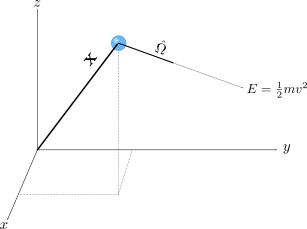
\includegraphics{transporte/neutron}
 \end{center}
\caption{\label{fig:neutron}Un neutrón individual (bola celeste), en un cierto tiempo~$t \in \mathbb{R}$ está caracterizado por la posición~$\vec{x}\in \mathbb{R}^3$ que ocupa en el espacio, por la dirección~$\omegaversor \in \mathbb{R}^2$ en la que viaja y por su energía cinética~$E\in\mathbb{R}$.}
\end{figure}

En la figura~\ref{fig:neutron} ilustramos un neutrón puntual que a un cierto tiempo~$t$ está ubicado en una posición espacial~$\vec{x}$ y se mueve en línea recta en una dirección~$\omegaversor$ con una energía~$E=1/2 \cdot m v^2$.

\section{Secciones eficaces} % WIP

{\color{red}\lipsum[3]}

\begin{definicion}
\label{def:sigmat}
La \emph{sección eficaz macroscópica total}~$\Sigma_t$ de un medio es tal que

\begin{equation*}
\Sigma_t \cdot dx 
\end{equation*}
%
es la probabilidad de que un neutrón tenga una colisión con el núcleo de algún átomo del material por el que viaja una distancia~$dx$ en línea recta. Es decir, la sección eficaz macroscópica es el número de colisiones esperadas por neutrón y por unidad de longitud lineal. Sus unidades son inversa de longitud, i.e. m$^{-1}$ ó cm$^{-1}$. 
\end{definicion}

Además de referirnos a la sección eficaz (ó XS por su terminología en inglés) total, podemos particularizar el concepto al tipo de reacción~$k$, es decir, \label{def:sigmak}$\Sigma_k \cdot dx$ es la probabilidad de que un neutrón tenga una reacción de tipo~$k$ en el intervalo~$dx$. En nuestro caso particular, la reacción genérica~$k$ puede ser particularizada a

\medskip

\begin{tabular}{cl}
 $t$ & total \\
 $c$ & captura radiativa \\
 $f$ & fisión \\
 $a$ & absorción ($\Sigma_c + \Sigma_f$) \\
 $s$ & dispersión (scattering)
\end{tabular}

\medskip

Las secciones eficaces macroscópicas dependen de la energía del neutrón incidente y de las propiedades del medio que provee los núcleos blanco. Como éstas dependen del espacio (usualmente a través de otras propiedades intermedias como por ejemplo temperaturas, densidades o concentraciones de impurezas), en general las secciones eficaces macroscópicas son funciones tanto del espacio~$\vec{x}$ como de la energía~$E$, es decir~$\Sigma_k = \Sigma_k(\vec{x}, E)$.

Una forma de incorporar el concepto de sección eficaz macroscópica es pensar que ésta proviene del producto de una sección eficaz microscópica~$\sigma_k$ y una densidad atómica~$n$ del medio

\begin{equation*}
 \Sigma_k = \sigma_k \cdot n
\end{equation*}


\begin{figure}[p]
 \begin{center}
  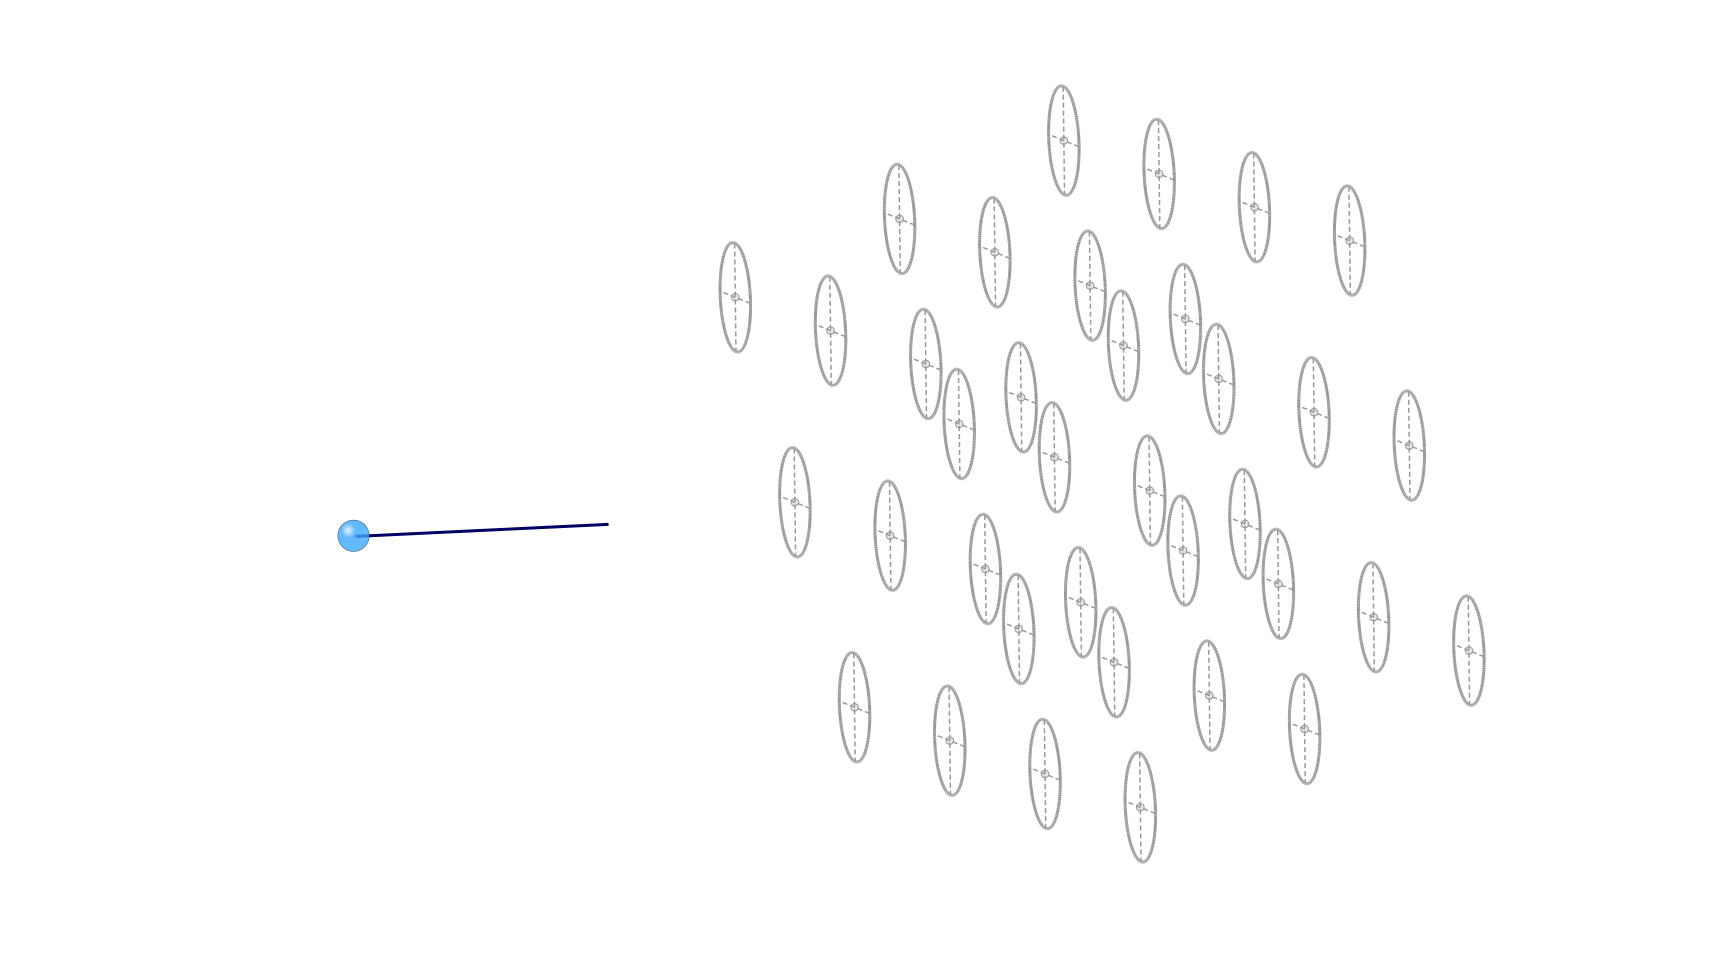
\includegraphics[width=0.7\linewidth]{transporte/xsmicro}
 \end{center}
\caption{\label{fig:xsmicro}Interpretación de la sección eficaz microscópica como el área asociada a un núcleo transversal a la dirección de viaje del neutrón incidente.}
\end{figure}

\begin{figure}[p]
 \begin{center}
  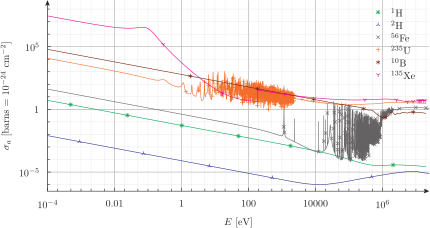
\includegraphics[width=\linewidth]{transporte/sigmas}
 \end{center}
\caption{\label{fig:sigmas}Dependencia de la sección eficaz microscópica de absorción~$\sigma_a$ con respecto a la energía~$E$ del neutrón incidente para diferentes isótopos blanco.}
\end{figure}

La magnitud~$\sigma_k$ tiene unidades de área (típicamente del orden de $10^{-24}~\text{cm}^2$, unidad que llamamos \emph{barn}\footnote{Se dice que durante las primeras mediciones experimentales de secciones eficaces los físicos americanos esperaban encontrar resultados del orden de las áreas transversales asociadas a los tamaños geométricos de los núcleos. Pero encontraron valores mucho más grandes, por lo que decían a modo de broma {“\foreignlanguage{english}this cross section is as big as a barn.”}}) y se interpreta como el área asociada a un núcleo transversal a la dirección de viaje de un neutrón tal que si este neutrón pasara a través de dicha área, se llevaría a cabo una reacción de tipo~$k$ (figura~\ref{fig:xsmicro}). Las secciones eficaces microscópicas dependen no solamente de las propiedades nucleares de los núcleo blanco sino que también dependen fuertemente de la energía~$E$ del neutrón incidente, llegando a cambiar varios órdenes de magnitud debido a efectos de resonancias como podemos observar en la figura~\ref{fig:sigmas}. Además, $\sigma_k$ depende de la temperatura~$T$ del medio que define la forma en la cual los átomos se mueven por agitación térmica alrededor de su posición de equilibrio ya que se produce un efecto tipo Doppler entre el neutrón y el núcleo blanco que modifica la sección eficaz microscópica~\cite{aatn-doppler-2013,aatn-doppler-2014}. Por lo tanto, para un cierto isótopo, $\sigma_k = \sigma_k(E,T)$.

Por otro lado, la densidad atómica~$n$ del medio depende de la densidad termodinámica~$\rho$, que a su vez depende de su estado termodinámico usualmente definido por la presión~$p$ y la temperatura~$T$. Como estas variables pueden depender de forma arbitraria del espacio~$\vec{x}$, podemos escribir efectivamente

\begin{equation*}
 \Sigma_k = n \cdot \sigma_k = n \Big( p(\vec{x}), T(\vec{x}) \Big) \cdot \sigma_k \Big(E, T(\vec{x}) \Big) = \Sigma_k (\vec{x}, E)
\end{equation*}

Las ideas presentadas son válidas para un único isótopo libre de cualquier influencia externa. En los reactores nucleares reales, por un lado existen efectos no lineales como por ejemplo el hecho de los átomos de hidrógeno o deuterio y los de oxígeno no están libres en la molécula de agua, que hacen que las secciones eficaces de el todo (i.e. de un conjunto de átomos enlazados covalentemente) no sean iguales a la suma algebraica de las partes y debamos calcular las secciones eficaces macroscópicas con una metodología más apropiada (ver sección~\ref{sec:evaluacionxs} y referencia~\cite{methods}). Por otro lado, justamente en los reactores nucleares las reacciones que interesan son las que dan como resultado la transmutación de materiales por lo que continuamente la densidad atómica~$n$ de todos los isótopos varía con el tiempo. En este trabajo, no vamos a tratar con la dependencia de las secciones eficaces con el tiempo explícitamente sino que llegado el caso, como discutimos en la sección~\ref{sec:multiescala}, daremos la dependencia implícitamente a través de otras propiedades intermedias tales como la evolución del quemado del combustible y/o la concentración de xenón~135 en la matriz de dióxido de uranio.

\medskip

A partir de este momento suponemos que conocemos las secciones eficaces macroscópicas en función del vector posición~$\vec{x}$ para todos los problemas que planteamos.

\subsection{Dispersión de neutrones} % DONE
\label{sec:scattering}

Cuando un neutrón que viaja en una cierta dirección~$\omegaversor$ con una energía~$E$ colisiona con un núcleo blanco en una reacción de dispersión o \emph{scattering}, tanto el neutrón como el núcleo blanco intercambian energía. En este caso podemos pensar que luego de la colisión, el neutrón incidente se ha transformado en otro neutrón emitido en una nueva dirección~$\omegaprimaversor$ con una nueva energía~$E^\prime$. Para tener este efecto en cuenta, utilizamos el concepto que sigue.

\begin{definicion}
\label{def:sigmasdif}
La \emph{sección eficaz de scattering diferencial}~$\Sigma_s$ tal que

\begin{equation*}
\Sigma_s(\vec{x}, \omegaversor \rightarrow \omegaprimaversor, E \rightarrow E^\prime) \, d\omegaprimaversor \, dE^\prime 
\end{equation*}
%
es la probabilidad por unidad de longitud lineal que un neutrón de energía~$E$ viajando en la dirección~$\omegaversor$ sea dispersado hacia un intervalo de energía entre~$E^\prime$ y~$E^\prime + dE^\prime$ y a un cono~$d\omegaprimaversor$ alrededor de la dirección~$\omegaprimaversor$.
\end{definicion}

Utilizando argumentos de simetría, podemos demostrar que la sección eficaz diferencial de scattering~$\Sigma_s$ sólo depende del producto interno~$\mu = \omegaversor \cdot \omegaprimaversor$ y no separadamente de~$\omegaversor$ y de~$\omegaprimaversor$ (figura~\ref{fig:omegamu}). Entonces podemos escribir la dependencia como~$\Sigma_s(\vec{x}, \omegaversor \rightarrow \omegaprimaversor, E \rightarrow E^\prime)$ ó como~$\Sigma_s(\vec{x}, \mu, E \rightarrow E^\prime)$, siempre y cuando tengamos en cuenta que

\begin{equation*}
\int_{4\pi} \Sigma_s(\vec{x}, \omegaversor \rightarrow \omegaprimaversor, E \rightarrow E^\prime) \, d\omegaprimaversor = 
\int_{-1}^{1} \Sigma_s(\vec{x}, \mu, E \rightarrow E^\prime) \, d\mu
\end{equation*}
%
lo que implica que
\begin{equation*}
 \Sigma_s(\vec{x}, \mu, E \rightarrow E^\prime) = 2\pi \, \Sigma_s(\vec{x}, \omegaversor \rightarrow \omegaprimaversor, E \rightarrow E^\prime)
\end{equation*}

Este abuso de notación es histórico y susceptible de provocar confusiones. Al escribir la probabilidad de scattering de~$\omegaversor$ hacia~$\omegaprimaversor$ sólo en función del producto interno~$\mu$ estamos teniendo en cuenta todas las posibles direcciones de salida tales que~$\mu  = \omegaversor \cdot \omegaprimaversor$.
Como podemos observar en la figura~\ref{fig:omegamu}, esto es~$2\pi$ veces la probabilidad de que el neutrón sea dispersado en la dirección~$\omegaprimaversor$ solamente. En los párrafos siguiente explícitamente diferenciamos uno de otro caso.

\begin{figure}[bh]
 \begin{center}
  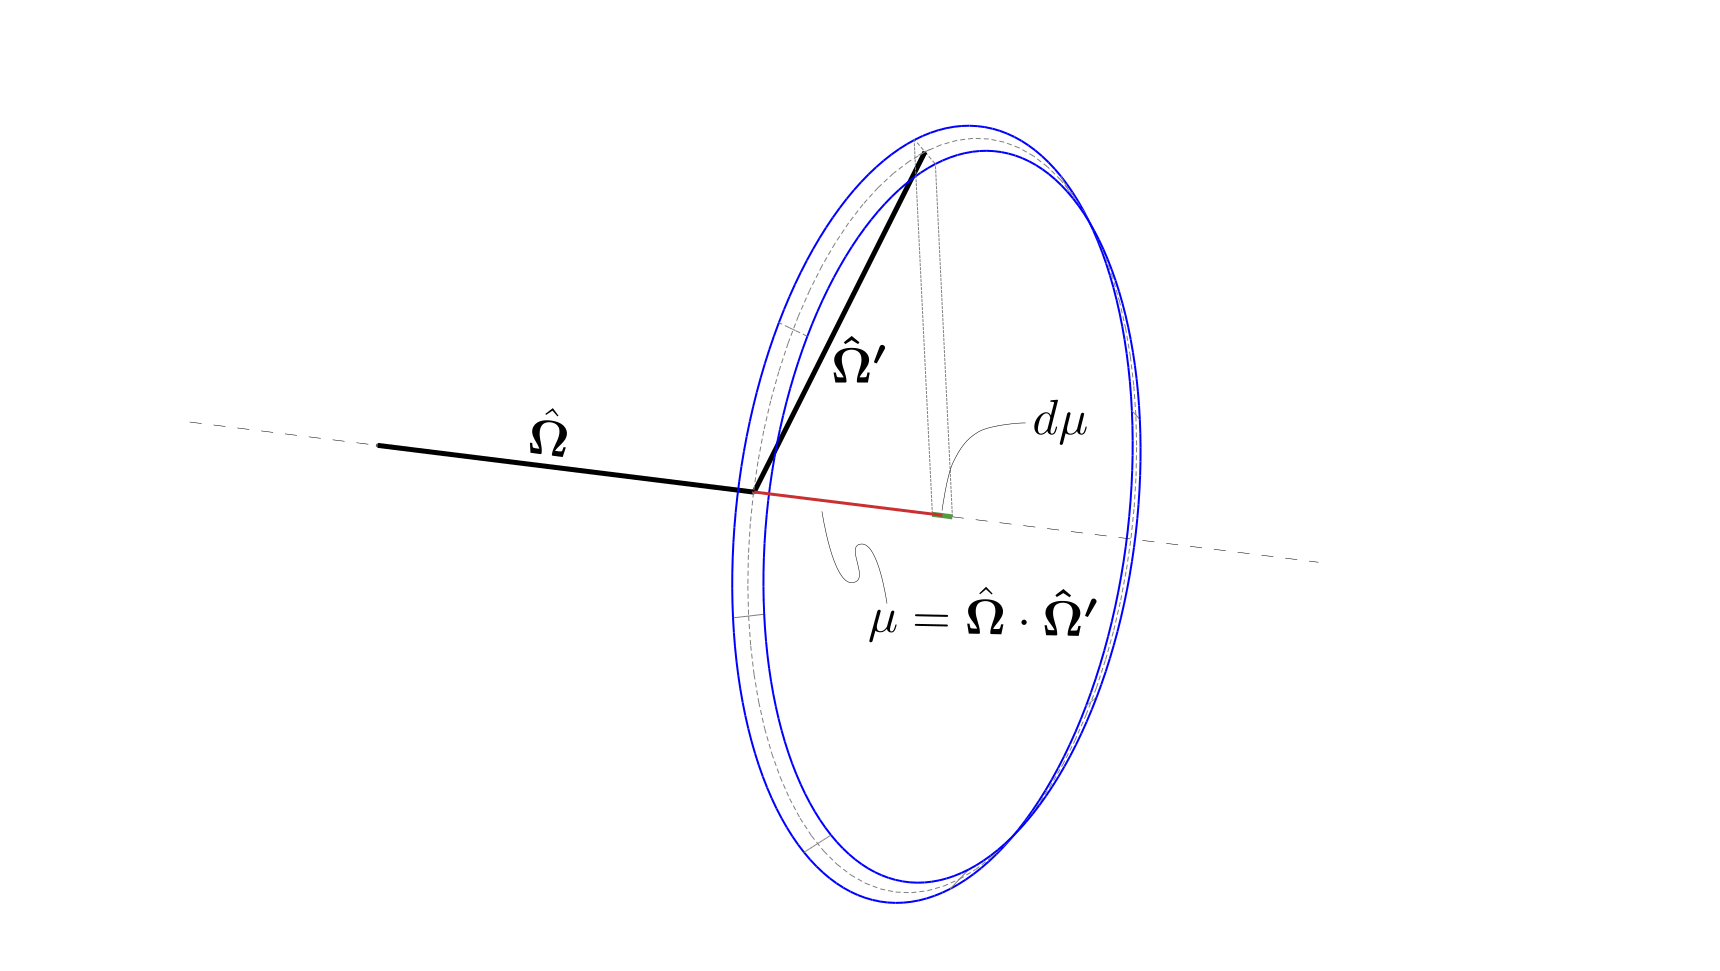
\includegraphics[width=0.6\linewidth]{transporte/omegamu-nice}
 \end{center}
\caption{\label{fig:omegamu}Debido a la simetría azimutal, el scattering no depende de las direcciones~$\omegaversor$ y de~$\omegaprimaversor$ en forma separada sino que depende del coseno del ángulo entre ellas~$\mu = \omegaversor \cdot \omegaprimaversor$.}
\end{figure}


\bigskip

En general podemos separar a la sección eficaz diferencial en una sección eficaz total~$\Sigma_{s_t}$ y en una probabilidad de distribución angular y energética~$f_s$ tal que

\begin{equation}
\label{eq:sigmastomega}
 \Sigma_s(\vec{x}, \omegaversor \rightarrow \omegaprimaversor, E \rightarrow E^\prime) = \Sigma_{s_t}(\vec{x}, E) \cdot f_s(\omegaversor \rightarrow \omegaprimaversor, E \rightarrow E^\prime)
\end{equation}
%
ó bien

\begin{equation}
\label{eq:sigmastmu}
 \Sigma_s(\vec{x}, \mu, E \rightarrow E^\prime) = \Sigma_{s_t}(\vec{x}, E) \cdot f_s(\mu, E \rightarrow E^\prime)
\end{equation}

% En esta expresión, el miembro izquierdo tiene unidades de longitud inversa por ángulo sólido inverso por energía inversa (por ejemplo $\text{cm}^-1 \cdot \text{stereoradián}^{-1} \cdot \text{eV}^{-1}$).
En ambos casos, $\Sigma_{s_t}$ es la sección eficaz macroscópica \emph{total} de scattering, que da la probabilidad por unidad de longitud de que un neutrón de energía~$E$ inicie un proceso de scattering. La función~$f_s$ describe la distribución de neutrones emergentes. Podemos integrar ambos miembros de las ecuaciones~\eqref{eq:sigmastomega} y~\eqref{eq:sigmastmu} con respecto a~$E^\prime$, y a~$\omegaprimaversor$ y a~$\mu$ respectivamente, y despejar~$\Sigma_{s_t}$ para obtener su definición

\begin{equation*}
 \Sigma_{s_t}(\vec{x}, E) =
\frac{\displaystyle \int_{0}^\infty \int_{4\pi} \Sigma_s(\vec{x}, \omegaversor \rightarrow \omegaprimaversor, E \rightarrow E^\prime) \, d\omegaprimaversor \, dE^\prime}
{\displaystyle \int_{0}^\infty \int_{4\pi} f_s(\omegaversor \rightarrow \omegaprimaversor, E \rightarrow E^\prime) \, d\omegaprimaversor \, dE^\prime} 
=
\frac{\displaystyle \int_{0}^\infty \int_{-1}^{1} \Sigma_s(\vec{x}, \mu, E \rightarrow E^\prime) \, d\mu \, dE^\prime}
{\displaystyle \int_{0}^\infty \int_{-1}^{1} f_s(\mu, E \rightarrow E^\prime) \, d\mu \, dE^\prime} 
\end{equation*}

El denominador es igual a la cantidad de partículas emitidas luego de la reacción, que para el caso del scattering es igual a uno. Luego

\begin{equation}\label{eq:sigmast}
 \Sigma_{s_t}(\vec{x}, E) =
 \int_{0}^\infty \int_{4\pi} \Sigma_s(\vec{x}, \omegaversor \rightarrow \omegaprimaversor, E \rightarrow E^\prime) \, d\omegaprimaversor \, dE^\prime
 =
 \int_{0}^\infty \int_{-1}^{1} \Sigma_s(\vec{x}, \mu, E \rightarrow E^\prime) \, d\mu \, dE^\prime 
\end{equation}


\medskip

Para tener en cuenta la dependencia de~$\Sigma_s$ con~$\mu$ (en realidad de~$f_s$ con~$\mu$) podemos recurrir a una expansión en polinomios de Legendre~(figura~\ref{fig:legendre}). En efecto, para dos energías~$E$ y~$E^\prime$ fijas,~$\Sigma_s$ depende de un único escalar~$-1 \leq \mu \leq 1$ sin presentar singularidades (i.e. es una función de cuadrado integrable) por lo que podemos escribir en una base ortogonal de polinomios%
%
\footnote{La definición particular de la expansión en polinomios de Legendre de la ecuación~\eqref{eq:sigmalegendremu} es tal que sea consistente con los usos y costumbres históricos de la evaluación de secciones eficaces (sección~\ref{sec:evaluacionxs}) y de códigos de celda (sección~\ref{sec:celda}). Es posible dar otra definición y desarrollar consistentemente la matemática para llegar a las mismas ecuaciones finales, pero ello modificaría la definición de los coeficientes de la expansión dados por la ecuación~\eqref{eq:coeflegendreomega} y haría que las secciones eficaces calculadas a nivel de celda no puedan ser introducidas directamente en la entrada del código de núcleo que describimos en el capítulo~\ref{cap:implementacion}. En particular, arribar a la ecuación~\eqref{eq:sigmas0} es de interés para la consistencia de las secciones eficaces entre códigos de diferente nivel. Por ejemplo, la referencia~\cite{lewis} utiliza otra forma de expandir el kernel de scattering que resulta en un factor dos de diferencia con respecto a la ecuación~\eqref{eq:coeflegendreomega}.}

\begin{figure}[bt]
\begin{center}
\includegraphics{transporte/legendre}
\end{center}
\caption{\label{fig:legendre}Primeros seis polinomios de Legendre~$P_\ell(\mu)$, $\ell = 1,\dots,6$. En el apéndice~\ref{ap:legendre} damos la definición matemática y otras propiedades interesantes de estos polinomios.}
\end{figure}

\begin{equation}\label{eq:sigmalegendremu}
\Sigma_s(\vec{x}, \mu, E \rightarrow E^\prime) = \sum_{\ell=0}^{\infty} \frac{2\ell + 1}{2} \, \Sigma_{s_\ell}(\vec{x}, E \rightarrow E^{\prime}) \cdot P_\ell(\mu)  
\end{equation}
%
donde los coeficientes resultan ser
\begin{equation}\label{eq:coeflegendremu} 
 \Sigma_{s_\ell}(\vec{x}, E\rightarrow E^{\prime}) =
 \int_{-1}^{1} \Sigma_s(\vec{x}, \mu, E\rightarrow E^\prime) \cdot P_\ell(\mu) \, d\mu 
\end{equation}
%
dada la propiedad de ortogonalidad de la base de Legendre según la cual

\begin{equation*}
 \int_{-1}^{1} P_\ell(\mu) \cdot P_{\ell^\prime}(\mu) \, d\mu = \frac{2}{2\ell + 1} \cdot \delta_{\ell \ell^\prime}
\end{equation*}
%
siendo~$\delta_{\ell \ell^\prime}$ la Delta de Kronecker

\begin{equation*}
 \delta_{\ell \ell^\prime} =
\begin{cases}
 1 & \text{si $\ell = \ell^\prime$} \\
 0 & \text{si $\ell \neq \ell^\prime$} \\
\end{cases}
\end{equation*}

% 
% \begin{table}
% \begin{center}
%  \begin{tabular}{clccl}
% \hline
%   $P_0(\mu) =$ & $1$                      & \hspace{1cm} & $P_3(\mu) =$ & $\frac{1}{2}(5\mu^3-3\mu)$  \\ \\
%   $P_1(\mu) =$ & $\mu$                    & \hspace{1cm} & $P_4(\mu) =$ & $\frac{1}{8}(35\mu^4-30\mu^2+3)$  \\ \\
%   $P_2(\mu) =$ & $\frac{1}{2}(3\mu^2-1)$  & \hspace{1cm} & $P_5(\mu) =$ & $\frac{1}{8}(63\mu^5-70\mu^3+15\mu)$  \\
% \hline
%  \end{tabular}
% \end{center}
% \caption{\label{tab:legendre}Primeros seis polinomios de Legrende.}
% \end{table}

Para la dependencia con~$\omegaversor$ y~$\omegaprimaversor$, la expansión y los coeficientes son respectivamente

\begin{equation}\label{eq:sigmalegendreomega}
\Sigma_s(\vec{x}, \omegaversor \rightarrow \omegaprimaversor, E \rightarrow E^\prime) = \sum_{\ell=0}^{\infty} \frac{2\ell + 1}{4\pi} \, \Sigma_{s_\ell}(\vec{x}, E \rightarrow E^{\prime}) \cdot P_\ell(\omegaversor \cdot \omegaprimaversor)  
\end{equation}

\begin{equation}\label{eq:coeflegendreomega}
 \Sigma_{s_\ell}(\vec{x}, E\rightarrow E^{\prime}) =
 2\pi \int_{4\pi} \Sigma_s(\vec{x}, \omegaversor \rightarrow \omegaprimaversor, E\rightarrow E^\prime) \cdot P_\ell(\omegaversor \cdot \omegaprimaversor) \, d\omegaprimaversor
\end{equation}


\bigskip

Es interesante notar que~$\Sigma_{s_t}$ sólo depende de~$\Sigma_{s_0}$. En efecto, reemplazando la expansión dada por la ecuación~\eqref{eq:sigmalegendremu} en la ecuación~\eqref{eq:sigmast} tenemos

\begin{align*}
 \Sigma_{s_t}(\vec{x}, E) &=
 \int_{0}^{\infty} \int_{-1}^{1} \sum_{\ell=0}^{\infty} \frac{2\ell + 1}{2} \, \Sigma_{s_\ell}(\vec{x}, E \rightarrow E^{\prime}) \cdot P_\ell(\mu) \, d\mu \, dE^\prime \\
 &= 
\bigintsss_{0}^{\infty} \left[ \sum_{\ell=0}^{\infty} \frac{2\ell + 1}{2} \, \Sigma_{s_\ell}(\vec{x}, E \rightarrow E^{\prime}) \cdot \int_{-1}^{1} P_\ell(\mu) \, d\mu \right] \, dE^\prime 
\end{align*}


Como todos los polinomios de Legendre son impares con respecto al argumento~$\mu$ excepto~$P_0(\mu)=1$, la integral sobre~$\mu$ es cero para todo~$\ell >0$. Luego

\begin{equation}\label{eq:sigmastys0}
 \Sigma_{s_t}(\vec{x}, E) = 
\int_{0}^{\infty} \left[ \frac{2 \cdot 0 + 1}{2} \cdot \Sigma_{s_0}(\vec{x}, E \rightarrow E^{\prime}) \cdot 2 \right] dE^\prime
=
\int_{0}^{\infty} \Sigma_{s_0}(\vec{x}, E \rightarrow E^{\prime}) dE^\prime
\end{equation}


\bigskip

Para fijar ideas, supongamos que tenemos scattering isotrópico en el marco de referencia del laboratorio.\footnote{Una expresión más apropiada según la potencial aplicación industrial de los conceptos desarrollados en esta tesis sería “marco de referencia de \emph{la central nuclear}.”} Entonces~$\Sigma_s$ no depende de~$\mu$ y el único término diferente de cero en la ecuación~\eqref{eq:sigmalegendreomega} es~$\Sigma_{s_0}$ que contiene información sólo sobre el cambio de energía del neutrón con respecto a las condiciones de incidencia:

\begin{equation}\label{eq:sigmas0}
\Sigma_s(\vec{x}, \omegaversor \rightarrow \omegaprimaversor, E \rightarrow E^\prime) = \sum_{\ell=0}^{\infty} \frac{2\ell + 1}{4\pi} \, \Sigma_{s_\ell}(\vec{x}, E \rightarrow E^{\prime}) \cdot P_\ell(\omegaversor \cdot \omegaprimaversor)  
= 
\frac{1}{4\pi} \cdot \Sigma_{s_0}(\vec{x}, E\rightarrow E^\prime)
\end{equation}

\medskip

Si en cambio el scattering resulta ser completamente elástico e isotrópico en el marco de referencia del centro de masa del sistema compuesto por el neutrón incidente y el núcleo blanco (condición que se da si el blanco está fijo en el marco de referencia del reactor sin posibilidad de moverse por efectos térmicos), entonces a cada energía de salida~$E^\prime$ le corresponde un único ángulo de scattering~$\mu$ a través de las leyes clásicas de conservación de energía y momento lineal. Para la dependencia en ángulos de entrada y salida \cite{stammler} es

\begin{equation*}
 \Sigma_s(\vec{x}, \mu, E \rightarrow E^\prime) =
\begin{cases}
 \displaystyle \Sigma_{s_t}(\vec{x}, E) \cdot \frac{\delta(\mu - \mu_0)}{(1-\alpha)E}  & \text{para}~\alpha E < E^\prime < E \\
\hfill 0 \hfil & \text{de otra manera}
\end{cases}
\end{equation*}
%
mientras que para la dependencia del coseno del ángulo de scattering~\cite{lewis} es

\begin{equation*}
 \Sigma_s(\vec{x}, \omegaversor \rightarrow \omegaprimaversor, E \rightarrow E^\prime) =
\begin{cases}
 \displaystyle \Sigma_{s_t}(\vec{x}, E) \cdot \frac{\delta(\mu - \mu_0)}{2\pi(1-\alpha)E}  & \text{para}~\alpha E < E^\prime < E \\
\hfill 0 \hfil & \text{de otra manera}
\end{cases}
\end{equation*}
%
donde ahora~$\delta(x)$ es la distribución Delta de Dirac (no confundir con Kronecker) y

\begin{align*}
 \alpha(A) &= \frac{(A-1)^2}{(A+1)^2} \\
 \mu_0(A,E,E^\prime) &= \frac{1}{2} \left[ (A+1)\sqrt{\frac{E^\prime}{E}} - (A-1) \sqrt{\frac{E}{E^\prime}} \right]
\end{align*}
%
siendo~$A$ es el número de masa del núcleo blanco. Llamamos a la magnitud~$\mu_0$ coseno medio de la dispersión. Esta nomenclatura~$\mu_0$ es general pero la expresión matemática es particular para el caso de scattering elástico e isotrópico en el marco de referencia del centro de masa. En la ecuación~\eqref{eq:mu0} generalizamos la definición para cualquier tipo de scattering.

La expresión para el~$\ell$-ésimo coeficiente de la expansión en polinomios de Legendre para~$\alpha E < E^\prime < E$ según la ecuación~\eqref{eq:coeflegendremu} es

\begin{equation*}
\Sigma_{s_\ell}(\vec{x}, E \rightarrow E^\prime) = \frac{\Sigma_{s_t}(\vec{x}, E)}{(1-\alpha) E} \int_{-1}^{1} \delta(\mu - \mu_0) \cdot P_\ell(\mu) \, d\mu = \frac{\Sigma_{s_t}(\vec{x}, E) }{(1-\alpha) E} \cdot P_\ell(\mu_0)
\end{equation*}
%
por lo que

\begin{equation*}
\Sigma_s(\vec{x}, \mu, E \rightarrow E^\prime) =
\frac{\Sigma_{s_t}(\vec{x},E)}{(1 - \alpha) E} \cdot \sum_{\ell=0}^{\infty} \frac{2\ell + 1}{2} \cdot P_\ell(\mu_0) \cdot P_\ell(\mu)
\end{equation*}

Tomando los dos primeros términos, podemos aproximar

\begin{equation*}
% \label{eq:mu01}
\Sigma_s(\vec{x}, \mu, E \rightarrow E^\prime) \approx
\frac{\Sigma_{s_t}(\vec{x},E)}{(1 - \alpha) E} \cdot \left(1 + \frac{3 \cdot \mu_0 \cdot \mu}{2}\right)
\end{equation*}
%
para~$\alpha E < E^\prime < E$, y cero para $E^{\prime} < \alpha E$ ó~$E^\prime > E$. Estas dos ideas nos permiten introducir los siguientes conceptos.

\begin{definicion}
 Decimos que hay \emph{scattering isotrópico} (a partir de ahora siempre nos vamos a referir al marco de referencia del reactor) cuando los coeficientes de la expansión de la sección eficaz diferencial de scattering~$\Sigma_s(\vec{x}, \mu,  E \rightarrow E^\prime)$ en polinomios de Legendre son todos nulos excepto el correpondiente a~$\ell=0$. En este caso, la sección eficaz diferencial no depende del ángulo y vale la ecuación~\eqref{eq:sigmas0}:

\begin{equation}\tag{\ref{eq:sigmas0}}
 \Sigma_s(\vec{x}, \omegaversor \rightarrow \omegaprimaversor, E \rightarrow E^{\prime}) = \frac{1}{4\pi} \cdot \Sigma_{s_0}(\vec{x}, E \rightarrow E^{\prime})
\end{equation}

Si además de~$\Sigma_{s_0}$ resulta también~$\Sigma_{s_1}\neq 0$ entonces decimos que el scattering es \emph{linealmente anisotrópico}, y la sección eficaz diferencial es la suma de la sección eficaz total más un coeficiente por el coseno del ángulo de scattering:

\begin{equation}
\label{eq:scatteringanisotropico}
 \Sigma_s(\vec{x}, \omegaversor \rightarrow \omegaprimaversor, E \rightarrow E^{\prime}) = \frac{1}{4\pi} \cdot \left[ \Sigma_{s_0}(\vec{x}, E \rightarrow E^{\prime}) + 3 \cdot  \Sigma_{s_1}(\vec{x}, E \rightarrow E^{\prime}) \cdot \left ( \omegaversor \cdot \omegaprimaversor \right) \right] 
\end{equation}

Definimos además el \emph{coseno medio de la dispersión}~$\mu_0$ para una ley de dispersión general como

% \begin{equation*}
%  \mu_0(\vec{x}, E \rightarrow E^{\prime}) = \frac{\Sigma_{s_1}(\vec{x}, E \rightarrow E^{\prime})}{\Sigma_{s_0}(\vec{x}, E \rightarrow E^{\prime})}
% \end{equation*}

% \begin{equation}\label{eq:mu0}
%  \mu_0(\vec{x}, E) =
% \frac{\displaystyle \int_0^\infty \int_{-1}^{1} \mu \cdot \Sigma_{s}(\vec{x}, \mu, E \rightarrow E^{\prime}) \, d\mu \, dE^\prime}
%      {\displaystyle \int_0^\infty \int_{-1}^{1}           \Sigma_{s}(\vec{x}, \mu, E \rightarrow E^{\prime}) \, d\mu \, dE^\prime}
% =
% \frac{\displaystyle \int_0^\infty \int_{-1}^{1}           \Sigma_{s_1}(\vec{x}, \mu, E \rightarrow E^{\prime}) \, d\mu \, dE^\prime}
%      {\displaystyle \int_0^\infty \int_{-1}^{1}           \Sigma_{s_0}(\vec{x}, \mu, E \rightarrow E^{\prime}) \, d\mu \, dE^\prime}
% = \frac{\Sigma_{st1}}{\Sigma_{st0}} = \frac{\Sigma_{st1}}{\Sigma_{s_t}}
% \end{equation}

\begin{equation}\label{eq:mu0}
 \mu_0(\vec{x}, E) =
\frac{\displaystyle \int_0^\infty \int_{-1}^{1} \mu \cdot \Sigma_{s}(\vec{x}, \mu, E \rightarrow E^{\prime}) \, d\mu \, dE^\prime}
     {\displaystyle \int_0^\infty \int_{-1}^{1}           \Sigma_{s}(\vec{x}, \mu, E \rightarrow E^{\prime}) \, d\mu \, dE^\prime}
=
\frac{\displaystyle \int_0^\infty           \Sigma_{s_1}(\vec{x}, E \rightarrow E^{\prime}) \, dE^\prime}
     {\displaystyle \int_0^\infty           \Sigma_{s_0}(\vec{x}, E \rightarrow E^{\prime}) \, dE^\prime}
\end{equation}
\end{definicion}


\medskip

En el caso de scattering general, i.e. no necesariamente isotrópico en algún marco de referencia y no necesarimente elástico, debemos conocer o bien la dependencia explícita de~$\Sigma_s$ con~$\omegaversor \cdot \omegaprimaversor$ (que puede ser aproximada mediante evaluaciones discretas) o bien una cierta cantidad de coeficientes~$\Sigma_{s_\ell}$ de su desarrollo en polinomios de Legendre sobre~$\mu$. En esta tesis trabajamos a lo más con scattering linealmente anisotrópico, es decir, la sección eficaz diferencial de scattering está dada por la ecuación~\eqref{eq:scatteringanisotropico} y suponemos que conocemos tanto~$\Sigma_{s_0}$ como~$\Sigma_{s_1}$ en función del espacio y de las energías antes de resolver la ecuación de transporte a nivel de núcleo (ver sección~\ref{sec:multiescala}).

% \medskip
% 
% En algunas situaciones sólo se necesita la sección eficaz de scattering independientemente de los ángulos de entrada y de salida como una medida de la probabilidad de que un núcleo tenga una interacción de dispersión, por ejemplo para comparar con la probabilidad de que ocurran otras interacciones que involucren absorciones.
% 
% \begin{definicion}
% \label{def:sigmastot}
% La \emph{sección eficaz total de scattering} es tal que
% 
% \begin{equation*}
% \Sigma_s(\vec{x}, E \rightarrow E^\prime) \, dE^\prime
% \end{equation*}
% %
% es la probabilidad por unidad de longitud lineal que un neutrón de energía~$E$ viajando en cualquier dirección sea dispersado hacia un intervalo de energía entre~$E^\prime$ y~$E^\prime + dE^\prime$ independientemente de cual sea la dirección de salida. 
% \end{definicion}
% 
% Podemos calcular esta sección eficaz total como la integral sobre todos los posibles ángulos de salida~$\omegaversor^{\prime}$ y sobre todos los posibles ángulos de incidencia~$\omegaversor$ de la sección eficaz diferencial de scattering:
% 
% \begin{equation*}
%  \Sigma_s(\vec{x}, E \rightarrow E^{\prime}) = \int_{4\pi} \int_{4\pi} \Sigma_s(\vec{x}, \omegaversor \rightarrow \omegaprimaversor, E \rightarrow E^\prime) \, d\omegaversor^{\prime} \, d\omegaversor
% \end{equation*}


\subsection{Fisión de neutrones} % WIP
\label{sec:fision}

Cuando un núcleo pesado se fisiona en dos núcleos más pequeños, ya sea debido a una fisión espontánea o a una fisión inducida por la absorción de un neutrón, se liberan además de los productos de fisión propiamente dichos y radiación~$\gamma$ debida al reacomodamiento de los niveles energéticos de los nucleones que intervienen en la reacción, entre dos y tres neutrones. Llamamos~$\nu(\vec{x}, E)$ a la cantidad promedio de neutrones liberados por cada fisión, $2 < \nu < 3$, que depende de la energía~$E$ del neutrón incidente y de la composición del material combustible  el punto~$\vec{x}$.

Como ahora se emite más de un neutrón, utilizamos la nomenclatura~$\nu\Sigma_f$ para indicar, en el sentido de la ecuación~\eqref{eq:sigmastomega} sección anterior, la sección eficaz diferencial como un producto de una sección eficaz total y una distribución angular

\begin{equation*}
 \nu\Sigma_f(\vec{x}, \omegaversor \rightarrow \omegaprimaversor, E \rightarrow E^\prime) = \nu\Sigma_{f_t}(\vec{x}, E) \cdot f_f(\omegaversor \rightarrow \omegaprimaversor, E \rightarrow E^\prime)
\end{equation*}

La distribución en energía de los nuetrones nacidos por fisión está dada por el espectro de fisión~$\chi$, que definimos a continuación.

\begin{definicion}
\label{def:chi}
El \emph{espectro de fisión}~$\chi(E)$ es tal que

\begin{equation*}
\chi(E) \, dE
\end{equation*}
%
es la probabilidad de que un neutrón nacido en una fisión tenga una energía en el intervalo~$[E,E+dE]$. El espectro de fisión está normalizado de forma tal que

\begin{equation}\label{eq:chinorm}
 \int_{0}^{\infty} \chi(E) \, dE = 1
\end{equation}
\end{definicion}

Los neutrones de fisión nacen isotrópicamente en el marco de referencia del reactor independientemente de la energía~$E$ del neutrón incidente que la provocó (decimos que los neutrones de fisión no tienen \emph{memoria}) y además la energía~$E^\prime$ con la que emergen tampoco depende de la energía del~$E$ neutrón incidente. Luego~$f_f$ no depende ni de~$\omegaversor$ ni de~$\omegaprimaversor$ y podemos separar la función~$f_t$ en una cierta dependencia de~$E$ multiplicada por~$\chi(E^\prime)$

\begin{equation*}
 f_f(\omegaversor \rightarrow \omegaprimaversor, E \rightarrow E^\prime) = A(E) \cdot \chi(E^\prime)
\end{equation*}

Como la integral de~$f_f$ sobre todas las posibles energías~$E^\prime$ y ángulos~$\omegaprimaversor$ debe ser igual a la cantidad~$\nu$ de neutrones emitidos

\begin{equation*}
 \nu(E) = \int_0^\infty \int_{4\pi} f_f(\omegaversor \rightarrow \omegaprimaversor, E \rightarrow E^\prime) \, d\omegaprimaversor \, dE^\prime =
A(E) \cdot \int_0^\infty \int_{4\pi} \chi(E^\prime) \, d\omegaprimaversor \, dE^\prime
\end{equation*}

Teniendo en cuenta la normalización de~$\chi$ dada por la ecuación~\eqref{eq:chinorm}, resulta

\begin{equation*}
 A(E) = \frac{\nu(E)}{4\pi}
\end{equation*}
%
por lo que

\begin{equation}\label{eq:nusigmaf}
\nu\Sigma_f(\vec{x}, \omegaversor \rightarrow \omegaprimaversor, E \rightarrow E^\prime) = \frac{\chi(E^\prime)}{4\pi} \cdot \nu\Sigma_{f_t}(\vec{x}, E)
\end{equation}

\medskip

Durante la operación de un reactor, no todos los neutrones provenientes de la fisión aparecen en el mismo instante en el que se produce. Una cierta fracción~$\beta$ de todos los neutrones son producto del decaimiento radioactivo o bien de productos de fisión generados instantáneamente o bien de hijos de éstos. En cualquier caso, en cálculos transitorios es necesario distinguir entre la fracción~$1-\beta$ de neutrones instantáneos (\emph{prompt}) que aparecen en el mismo momento de la fisión y la fracción~$\beta$ de neutrones retardados que aparecen más adelante. Para ello dividimos a los neutrones retardados en~$I$ grupos, les asignamos una fracción~$\beta_i$ y una constante de tiempo~$\lambda_i$, para~$i=1,\dots,N$ y definimos un mecanismo de aparición exponencial para cada uno de ellos.

En cálculos estacionarios no es necesario realizar esta división entre neutrones instantáneos y retardados ya que eventualmente todos los neutrones estarán contribuyendo a la reactividad neta del reactor. En el caso particular en el que no hay una fuente externa de neutrones sino que todas las fuentes se deban a fisiones la probabilidad de que el reactor esté exactamente crítico es cero como discutimos en la sección~\ref{sec:problemas}. Para poder realizar cálculos estacionarios y además tener una idea de la distancia a la criticidad debemos recurrir a un reactor crítico asociado, cuya forma más usual es el \emph{reactor crítico asociado en~$k$}. En este caso, dividimos las fuentes de fisión se artificialmente por un número real~$k_\text{eff} \sim 1$ que pasa a ser una incógnita del problema y cuya diferencia con la unidad da una idea de la distancia a la criticidad del reactor original (ver sección~\ref{sec:problemas}).




\section{Flujos y ritmos de reacción} % WIP

El problema central del cálculo de reactores es la determinación de la distribución espacial y temporal de los neutrones dentro del núcleo de un rector nuclear. En esta sección desarrollamos la matemática para el caso de~$\vec{x} \in \mathbb{R}^3$. En casos particulares aclaramos cómo debemos proceder para problemas en una y en dos dimensiones.

{\color{red} \lipsum[18]}

Comenzamos con las siguientes definiciones.

\begin{definicion}
\label{def:N}
La \emph{distribución de densidad de neutrones}~$N$ en un espacio de las fases de siete dimensiones~$\vec{x} \in \mathbb{R}^3$, $\omegaversor \in \mathbb{R}^2$ (\footnote{Si bien la dirección~$\omegaversor = [ \Omega_x \, \Omega_y \, \Omega_z]^T$ tiene tres componentes, sólo dos son independientes (por ejemplo las coordenadas angulares cenital~$\theta$ y azimutal~$\varphi$) ya que debe cumplirse que~$\Omega_x^2 + \Omega_y^2 + \Omega_z^2 = 1$.}), $E \in \mathbb{R}$ y~$t \in \mathbb{R}$ tal que

\begin{equation*}
 N(\vec{x}, \omegaversor, E, t) \, d^3\vec{x} \, d\omegaversor \, dE
\end{equation*}
%
es el número de neutrones (en el sentido de la media estadística dada la naturaleza estocástica del comportamiento de los neutrones) en un elemento volumétrico~$d^3\vec{x}$ ubicado alrededor del punto~$\vec{x}$ del espacio viajando en el cono de direcciones de magnitud~$d\omegaversor$ alrededor de la dirección~$\omegaversor$ con energías entre~$E$ y~$E+dE$ en el tiempo~$t$.
\end{definicion}


\begin{definicion}
\label{def:flujoangular}
El \emph{flujo angular}~$\psi$ es el producto entre la velocidad y la distribución de densidad de los neutrones

\label{flujoangular}
\begin{align*}
 \psi(\vec{x}, \omegaversor, E, t) &= v(E) \cdot N(\vec{x}, \omegaversor, E, t)  \\
&= \sqrt{\frac{2E}{m}} \cdot N(\vec{x}, \omegaversor, E, t) 
\end{align*}
%
donde~$v(E)$ es la velocidad clásica correspondiente a un neutrón de masa~$m$ cuya energía cinética es~$E$.
\end{definicion}

Esta magnitud es más útil para evaluar ritmos de colisiones y reacciones que la densidad de neutrones~$N$. En efecto, como~$v \cdot dt$ es la distancia que viaja un neutrón de velocidad~$v$, entonces

\begin{equation*}
 \psi(\vec{x}, \omegaversor, E, t) \, d^3\vec{x} \, d\omegaversor \, dE \, dt = v(E) \cdot N(\vec{x}, \omegaversor, E, t) \, dt \,\,\, d^3\vec{x} \, d\omegaversor \, dE 
\end{equation*}
%
es el número total de longitudes lineales que los neutrones han viajado en la dirección~$\omegaversor$ con energía~$E$ que estaban en el tiempo~$t$ en la posición~$\vec{x}$. Como además~$\Sigma_k \cdot dx$ es la probabilidad de que un nuetrón tenga una reacción de tipo~$k$ en el intervalo~$dx$ (definición~\ref{def:sigmat}, página \pageref{def:sigmak}), entonces la expresión

\begin{equation*}
 \Sigma_k(\vec{x}, E) \cdot \psi(\vec{x}, \omegaversor, E, t) \, d^3\vec{x} \, d\omegaversor \, dE
\end{equation*}
%
es el número de reacciones de tipo~$k$ en el diferencial de volumen de fases~$d^3\vec{x} \, d\omegaversor \, dE$ debido a neutrones de energía~$E$ viajando en la dirección~$\omegaversor$ en el punto~$\vec{x}$ del espacio en el instante~$t$. Para obtener el número total de reacciones de todos los neutrones independientemente de la dirección~$\omegaversor$ del neutrón incidente debemos integrar esta cantidad sobre todos los posibles ángulos de incidencia. Para ello utilizamos el siguiente concepto.

\begin{definicion}
\label{def:flujoescalar}
El \emph{flujo escalar}~$\phi$ es la integral del flujo angular sobre todas las posibles direcciones de viaje de los neutrones:

\label{flujoescalar}
\begin{equation*}
\phi(\vec{x}, E, t) = \int_{4\pi} \psi(\vec{x}, \omegaversor, E, t) \, d\omegaversor
\end{equation*}
\end{definicion}

Con esta nomenclatura, el ritmo~$R_k$ de reacciones de tipo~$k$ en~$d^3\vec{x}\,dE$ es

\begin{equation*}
R_k (\vec{x}, E, t) \, d^3\vec{x} \, dE = \Sigma_k(\vec{x}, E) \cdot \phi(\vec{x}, E, t) \, d^3\vec{x} \, dE
\end{equation*}
%
con lo que el producto~$R_t = \Sigma_t \phi$ da una expresión simple para la distribución del ritmo de reacciones totales por unidad de volúmen y de energía, que es lo que buscábamos al introducir las ideas de flujo escalar y flujo angular.

\begin{definicion}
\label{def:corriente}
El \emph{vector corriente}~$\vec{J}$ es la integral del producto entre el flujo angular y el versor de dirección de viaje de los neutrones~$\omegaversor$ sobre todas las direcciones de viaje:

\label{vectorcorriente}
\begin{equation*}
 \vec{J}(\vec{x},E,t) = \int_{4\pi} \left[ \psi(\vec{x}, \omegaversor, E, t) \cdot \omegaversor \right] \, d\omegaversor
\end{equation*}
\end{definicion}

Debemos notar que esta magnitud es vectorial ya el integrando es un vector cuya magnitud es igual al flujo angular y cuya dirección es la del versor~$\omegaversor$ sobre el cual estamos integrando. El producto escalar entre el vector corriente~$\vec{J}$ y un cierto versor espacial~$\hat{\vec{n}}$

\begin{equation}
\label{eq:jn}
 J_n(\vec{x}, E, t) = \hat{\vec{n}} \cdot \vec{J}(\vec{x}, E, t) = \int_{4\pi} \psi(\vec{x}, \omegaversor, E, t) \cdot \left( \omegaversor \cdot \hat{\vec{n}} \right) \, d\omegaversor
\end{equation}
%
da el número neto de neutrones que cruzan un área unitaria perpendicular a~$\hat{\vec{n}}$ en la dirección positiva. Este número neto es la resta de dos contribuciones

\begin{equation*}
 J_n(\vec{x}, E, t) = J_n^+(\vec{x}, E, t) - J_n^-(\vec{x}, E, t)
\end{equation*}
%
donde

\begin{align}
 J_n^+(\vec{x},E,t) &= \int_{\omegaversor \cdot \hat{\vec{n}} > 0} \psi(\vec{x}, \omegaversor, E, t) \left(\omegaversor \cdot \hat{\vec{n}}\right) d\omegaversor \nonumber \\
\ J_n^-(\vec{x},E,t) &= \int_{\omegaversor \cdot \hat{\vec{n}} < 0} \psi(\vec{x}, \omegaversor, E, t) \left(\omegaversor \cdot \hat{\vec{n}}\right) d\omegaversor \label{eq:jnegativa}
\end{align}

\begin{figure}
\begin{center}
 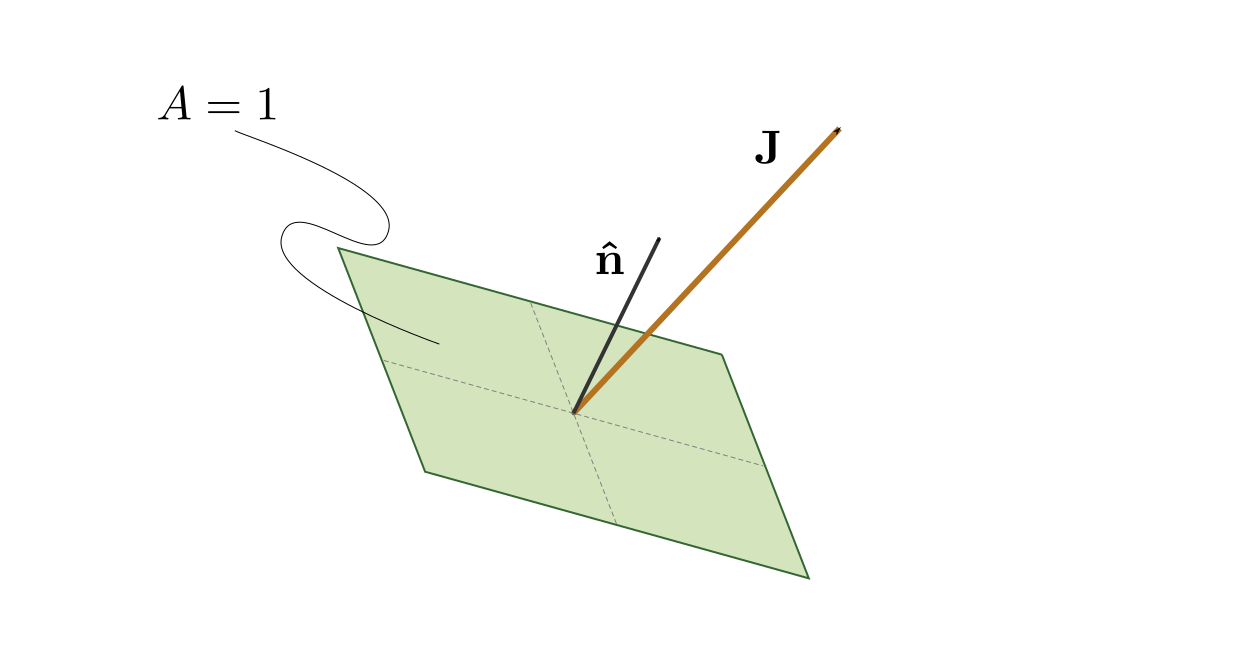
\includegraphics[width=0.5\linewidth]{transporte/normal}
\end{center}
\caption{\label{fig:normal}Interpretación del producto del vector corriente con el vector normal a una superficie como el número neto de neutrones que cruzan un área unitaria.}
\end{figure}


\section{Transporte de neutrones} % WIP

{\color{red}\lipsum[7]}

\subsection{Operador de transporte} % WIP

Consideremos un volumen finito~$V\in \mathbb{R}^3$ arbitrario fijo en el espacio y consideremos ahora otro volumen~$V^{\prime}(t)\in \mathbb{R}^3$ que se mueve en una dirección~$\omegaversor$ con una velocidad~$v(E)$ correspondiente a una energía~$E$, de tal manera que en el instante~$t$ ambos volúmenes coinciden. En ese momento, la cantidad de neutrones con dirección~$\omegaversor$ en torno al cono definido por~$d\omegaversor$ y con energías entre~$E$ y~$E+dE$ en el volumen~$V \equiv V^{\prime}(t)$ es

\begin{equation}
\label{eq:nv}
 N_V(\omegaversor, E, t) \, d\omegaversor \, dE = \left[ \int_{V \equiv V^{\prime}(t)} N(\vec{x}, \omegaversor, E, t) \, d^3\vec{x} \right] \, d\omegaversor \, dE
\end{equation}

Dado que la posición del dominio de integración cambia con el tiempo, la derivada total de esta magnitud con respecto al tiempo es la suma de una derivada parcial y una derivada material:

\begin{equation}
\label{eq:integral_dos_dominios}
 \frac{dN_V}{dt} = \frac{\partial N_V}{\partial t} +
\text{lim}_{\Delta t \rightarrow 0} \frac{1}{\Delta t} \left[ \int_{V^{\prime}(t+\Delta t)} N(\vec{x}, \omegaversor, E, t) \, d^3\vec{x}  - \int_{V^{\prime}(t)} N(\vec{x}, \omegaversor, E, t) \, d^3\vec{x} \right]
\end{equation}

Ahora necesitamos que el dominio de integración de la segunda integral sea igual al de la primera. Para ello, notamos que

\begin{equation*}
 \text{lim}_{\Delta t \rightarrow 0} V^{\prime}(t+\Delta t) = V^{\prime}(t) + v(E) \omegaversor \cdot \Delta t
\end{equation*}
%
para cada punto~$\vec{x} \in V^{\prime}(t)$. Además, como ni~$v(E)$ ni~$\hat{\Omega}_i$ para~$i=x,y,z$ dependen de~$\vec{x}$, entonces

\begin{equation*}
 \frac{\partial}{\partial x_i} \Big[ x_i + v(E) \, \hat{\Omega}_i \cdot \Delta t \Big] = 1
\end{equation*}
%
y podemos hacer un cambio de coordenadas unitario en la ecuación~\eqref{eq:integral_dos_dominios} para que el dominio de integración de la primera integral coincida entonces con el de la segunda y obtener así

\begin{equation*}
 \frac{dN_V}{dt} =  \frac{\partial N_V}{\partial t} +
\int_{V^{\prime}(t)} \text{lim}_{\Delta t \rightarrow 0} \frac{1}{\Delta t} \left[ N(\vec{x} + v(E)\omegaversor \cdot \Delta t, \omegaversor, E, t) - N(\vec{x}, \omegaversor, E, t) \right]  \, d^3\vec{x} 
\end{equation*}

Como el término entre corchetes es igual a~$v(E)$ veces la derivada espacial de la función~$N(\vec{x}, \omegaversor, E, t)$ en la dirección~$\omegaversor$ resulta

\begin{equation*}
 \text{lim}_{\Delta t \rightarrow 0} \frac{1}{\Delta t} \left[ N(\vec{x} + v(E)\omegaversor \cdot \Delta t, \omegaversor, E) - N(\vec{x}, \omegaversor, E)\right] \, d^3\vec{x}  = v(E) \left\{ \omegaversor \cdot \text{grad} \left[N(\vec{x}, \omegaversor, E)\right] \right\}
\end{equation*}
%
y $V^{\prime}(t) \equiv V$ entonces podemos escribir la derivada total de la cantidad de neutrones en~$V$ con respecto al tiempo como

\begin{equation*}
 \frac{dN_V}{dt} = \frac{\partial N_V}{\partial t} + v(E) \left\{ \int_{V} \omegaversor \cdot \text{grad} \left[ N(\vec{x}, \omegaversor, E, t) \right]  d^3\vec{x} \right\}
\end{equation*}

Teniendo en cuenta la ecuación~\eqref{eq:nv} y la definición~\ref{def:flujoangular} de flujo angular~$\psi$

\begin{equation*}
 \frac{d}{dt} \int_{V} N(\vec{x}, \omegaversor, E, t) \, d^3\vec{x}  = \int_{V} \left\{ \frac{1}{v} \frac{\partial \psi}{\partial t} + \omegaversor \cdot \text{grad} \left[ \psi(\vec{x}, \omegaversor, E, t) \right] \right\}  d^3\vec{x}
\end{equation*}
%
donde notamos que el gradiente opera sólo sobre las componentes espaciales, es decir

\begin{equation*}
 \text{grad} \left[ \psi(\vec{x}, \omegaversor, E, t) \right] =
\begin{bmatrix}
 \displaystyle \frac{\partial \psi}{\partial x} \\ \\
 \displaystyle \frac{\partial \psi}{\partial y} \\ \\
 \displaystyle \frac{\partial \psi}{\partial z} \\
\end{bmatrix}
\end{equation*}

\subsection{Operador de producciones} % WIP

Habiendo estudiado la expresión matemática que describe el transporte de neutrones, pasamos ahora a estudiar la forma en la que se producen. Los neutrones pueden aparecer en un diferencial de espacio de las fases~$d\vec{x} \, d\omegaversor \, dE \, dt$ debido a uno de los siguiente tres mecanismos, que analizamos a continuación: scattering, fisión y fuentes externas.

\subsubsection{Fuente por scattering} % WIP

Un neutrón que viajando con una energía~$E^\prime$ y una dirección~$\omegaprimaversor$ sufre una colisión de scattering en el punto~$\vec{x}$ y emerge con una energía~$E$ y una dirección~$\omegaversor$ es efectivamente una fuente de neutrones en~$d\vec{x} \,  d\omegaversor \, dE \, dt$ debido a scattering. Esta fuente~$q_s$ debe ser entonces igual al producto de la probabilidad por unidad de longitud de recorrido de neutrones que viajando en con una energía~$E^\prime$ en una dirección~$\omegaprimaversor$ colisionen con un núcleo blanco en el punto~$\vec{x}$ y como resultado adquieren una dirección de viaje~$\omegaversor$ y una energía~$E$ (ver sección~\ref{sec:scattering}) por la cantidad de longitudes lineales viajadas, teniendo en cuenta todos los posibles valores de~$\omegaprimaversor$ y de~$E^\prime$. Es decir

\begin{equation}
\label{eq:qs}
\int_V
q_s(\vec{x}, \omegaversor, E, t)
\, d^3\vec{x} = 
\int_V
 \int_{0}^{\infty} \int_{4\pi} \Sigma_s(\vec{x}, \omegaprimaversor  \rightarrow \omegaversor, E^\prime \rightarrow E) \cdot \psi(\vec{x}, \omegaprimaversor, E^\prime, t) \, d\omegaprimaversor \, dE^\prime
\, d^3\vec{x}
\end{equation}

Debemos notar que en esta ecuación hemos invertido el índice de las variables primadas con respecto a la sección~\ref{sec:scattering}, inversión que mantendremos a lo largo de esta sección.

\subsubsection{Fuente por fisión} % WIP

Los neutrones que nacen por fisiones de núcleos de materiales combustibles en el punto~$\vec{x}$ lo hacen isotrópicamente y con una cierta distribución energética~$\chi(E)$ (ver sección~\ref{sec:fision}). Como también discutimos en la página~\pageref{sec:fision}, debemos calcular la fuente de fisión ligeramente diferente si se trata de un problema transitorio, estacionario con fuente o estacionario sin fuente. Sin pérdida de generalidad, para fijar ideas supongamos que desde el punto de vista de la fisión el problema es estacionario con fuente. La tasa de generación de neutrones debidas a fisión es el producto del número probable de nacimientos en~$\vec{x}$ con energías entre~$E$ y~$E+dE$ por unidad de longitud de recorrido de neutrones que viajando con dirección~$\omegaversor$ y energía~$E$ generan la fisión del núcleo pesado en el punto~$\vec{x}$ debido a neutrones incidentes con dirección de viaje~$\omegaprimaversor$ y energía incidente~$E^\prime$ (ver sección~\ref{sec:fision}) por la cantidad de longitudes lineales viajadas, teniendo en cuenta todos los posibles valores de~$\omegaprimaversor$ y de~$E^\prime$:

\begin{align}\label{eq:qf}
\int_V
q_f(\vec{x}, \omegaversor, E, t)
\, d^3\vec{x} &= 
\int_V
\frac{\chi(E)}{4\pi} \int_{0}^{\infty} \int_{4\pi} \nu\Sigma_f(\vec{x}, E^\prime) \cdot \psi(\vec{x}, \omegaprimaversor, E^\prime, t) \, d\omegaprimaversor \, dE^\prime
\, d^3\vec{x} \nonumber \\
 &= 
\int_V
\frac{\chi(E)}{4\pi} \int_{0}^{\infty} \nu\Sigma_f(\vec{x}, E^\prime) \cdot \phi(\vec{x}, E^\prime, t) \, dE^\prime
\, d^3\vec{x}
\end{align}

\subsubsection{Fuente independiente} % WIP

Por último, para no perder generalidad tenemos que tener en cuenta las fuentes externas de neutrones, i.e. aquellas que no provienen de la fisión de materiales presentes en el núcleo sino de otras fuentes totalmente independientes como puede ser una fuente de americio-berilio. Matemáticamente, las modelamos como la integral sobre el volumen~$V$ de una función conocida~$s(\vec{x}, \omegaversor, E, t)$ del espacio, la dirección, la energía y el tiempo que representa la cantidad de neutrones emitidos con energía~$E$ en el punto~$\vec{x}$ con dirección~$\omegaversor$ en el instante~$t$.

\subsection{La ecuación de transporte} % WIP

La conservación de neutrones implica que la derivada temporal total de cualquier magnitud relacionada a la distribución espacial de neutrones debe ser igual a la diferencia entre la tasa de producciones y la tasa de desapariciones. El ritmo de aparición de neutrones en el volumen~$V$ con energías entre~$E$ y~$E+dE$ en un cono~$d\omegaversor$ alrededor de la dirección~$\omegaversor$ es

\begin{equation*}
\int_V
 q(\vec{x}, \omegaversor, E, t)  \, dE \, d\omegaversor
\, d^3\vec{x}
 =
\int_V
 \left [q_s(\vec{x}, \omegaversor, E, t) + q_f(\vec{x}, \omegaversor, E, t) + s(\vec{x}, \omegaversor, E, t) \right]  \, dE \, d\omegaversor
\, d^3\vec{x}
\end{equation*}

El ritmo con el que desaparecen los neutrones de energía~$E$ viajando en la dirección~$\omegaversor$ en el volumen~$V$ es

\begin{equation*}
\int_V
R_t(\vec{x}, \omegaversor, E, t)  \, dE \, d\omegaversor
\, d^3\vec{x}
 =
\int_V
\Sigma_t(\vec{x}, E) \cdot \psi(\vec{x}, \omegaversor, E, t) \, dE \, d\omegaversor
\, d^3\vec{x}
\end{equation*}
%
por lo que

\begin{multline}
% \label{eq:transporteqintegral}
\left( \int_{V} \left\{ \frac{1}{v} \frac{\partial \psi}{\partial t} + \omegaversor \cdot \text{grad} \left[ \psi(\vec{x}, \omegaversor, E, t) \right] \right\}  d^3\vec{x} \right) \, dE \, d\omegaversor = \\
\left( \int_{V} q(\vec{x}, E, \omegaversor, t) \, d^3\vec{x} \right) \, dE \, d\omegaversor -
\left( \int_{V} \Sigma_t(\vec{x}, E) \cdot \psi(\vec{x}, \omegaversor, E, t) \, d^3\vec{x} \right) \, dE \, d\omegaversor
\end{multline}


Como el dominio de integración~$V$ es arbitrario, la igualdad debe cumplirse punto a punto

\begin{equation}
\label{eq:transporteq}
 \frac{1}{v} \frac{\partial}{\partial t} \left[ \psi(\vec{x}, \omegaversor, E, t) \right]
 + \omegaversor \cdot \text{grad} \left[ \psi(\vec{x}, \omegaversor, E, t) \right]
 + \Sigma_t(\vec{x}, E) \cdot \psi(\vec{x}, \omegaversor, E, t)
 = q(\vec{x}, \omegaversor, E, t)
\end{equation}

Desarrollando el término de fuente en sus tres términos y teniendo en cuenta que la relación entre velocidad y energía es la clásica~$E=mv^2/2$, llegamos a la \emph{ecuación de transporte de neutrones}

\begin{multline}
\label{eq:transporte}
 \sqrt{\frac{m}{2E}} \frac{\partial}{\partial t} \left[ \psi(\vec{x}, \omegaversor, E, t) \right]
 + \omegaversor \cdot \text{grad} \left[ \psi(\vec{x}, \omegaversor, E, t) \right]
 + \Sigma_t(\vec{x}, E) \cdot \psi(\vec{x}, \omegaversor, E, t) = \\
 \int_{0}^{\infty} \int_{4\pi} \Sigma_s(\vec{x}, \omegaprimaversor \rightarrow \omegaversor, E^\prime \rightarrow E) \cdot \psi(\vec{x}, \omegaprimaversor, E^\prime, t) \, d\omegaprimaversor \, dE^\prime \\
+ \frac{\chi(E)}{4\pi} \int_{0}^{\infty} \int_{4\pi} \nu\Sigma_f(\vec{x}, E^\prime) \cdot \psi(\vec{x}, \omegaprimaversor, E^\prime, t) \, d\omegaprimaversor \, dE^\prime 
+ s(\vec{x}, \omegaversor, E, t)
\end{multline}
%
que es una ecuación diferencial en derivadas parciales de primer orden en el espacio (debemos recordar que el operador gradiente opera sólo sobre las coordenadas espaciales) y de primer orden en el tiempo para la incógnita~$\psi$ sobre el espacio~$\vec{x}$, la dirección~$\omegaversor$, la energía~$E$ y el tiempo~$t$. Las secciones eficaces~$\Sigma_t$ y~$\nu\Sigma_f$ son distribuciones conocidas del espacio y de la energía, como también lo es la fuente~$s$ con una dependencia adicional sobre la dirección. La sección eficaz diferencial de scattering~$\Sigma_s$ debe ser conocida en su dependencia tanto en la energía incidente~$E^\prime$ como en la energía saliente~$E$ y en el coseno del ángulo de scattering~$\mu = \omegaprimaversor \cdot \omegaversor$, usualmente dada como coeficientes~$\Sigma_{s_\ell}$ de expansión en polinomios de Legendre sobre el escalar~$\mu$. El parámetro~$m$ es la masa en reposo del neutrón.


\subsection{Evaluación del término de scattering} % WIP

Prestemos atención al término de fuente por scattering dado por la ecuación~\eqref{eq:qs}. Dado que hemos supuesto que la sección eficaz diferencial de scattering esté definida por los coeficientes del desarrollo en polinomios de Legendre~$\Sigma_{s_\ell}$ introducidos en la ecuación~\eqref{eq:sigmalegendreomega} (recordar que seguimos invirtiendo las variables primadas), entonces podemos escribir el término de scattering como

\begin{equation}
\label{eq:qs1}
q_s(\vec{x}, \omegaversor, E, t) =
 \sum_{\ell=0}^{\infty} \frac{ 2\ell + 1}{4\pi} \cdot
\int_{0}^{\infty} \left[ \Sigma_{s_\ell}(\vec{x}, E^{\prime} \rightarrow E) \int_{4\pi} P_\ell(\omegaversor \cdot \omegaprimaversor) \cdot \psi(\vec{x}, \omegaprimaversor, E^\prime,t)\, d\omegaprimaversor \right] \, dE^{\prime}
\end{equation}

Si bien esta expresión ya es suficiente para evaluar el término de scattering cuando tenemos su desarrollo de Legendre, podemos ahondar un poco más en la estructura de la ecuación de transporte desarrollando en una base apropiada el flujo angular, de la misma manera en la que desarrollamos~$\Sigma_s$ en una serie de polinomios de Legendre sobre el parámetro~$\mu = \omegaversor \cdot \omegaprimaversor$. Para ello, notamos que~$\psi$ depende angularmente de un versor dirección~$\omegaversor = [\hat\Omega_x \, \hat\Omega_y \, \hat\Omega_z]^T$ (u~$\omegaprimaversor$ en el caso de la ecuación~\eqref{eq:qs1}). Esta vez, la base de expansión apropiada es la dada por los armónicos esféricos reales (figura~\ref{fig:harmonics}). En efecto, podemos escribir cualquier función~$f(\hat\Omega_x, \hat\Omega_y, \hat\Omega_z)$ de cuadrado integrable, con $\hat\Omega_x^2 + \hat\Omega_y^2 + \hat\Omega_z^2 = 1$, como

\begin{figure}[t]
 \begin{center}
  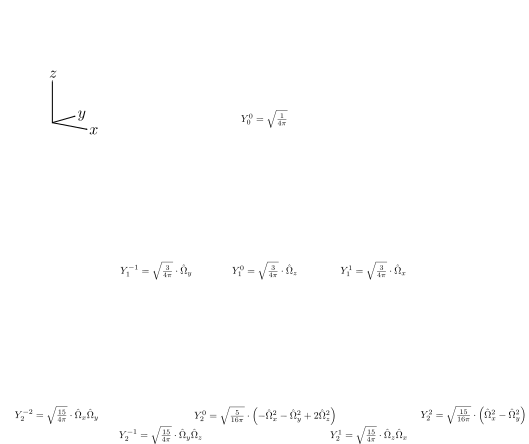
\includegraphics{transporte/harmonics}
 \end{center}
\caption{\label{fig:harmonics}Los primeros nueve armónicos esféricos reales. Ver apéndice~\ref{ap:armonicos} para una lista completa y la figura~\ref{fig:armonicoswiki} para una representación visual alternativa.}
\end{figure}


\begin{equation*}
f(\hat\Omega_x, \hat\Omega_y, \hat\Omega_z) = \sum_{\ell=0}^\infty \sum_{m=-\ell}^\ell f_\ell^m \cdot Y_\ell^m(\hat\Omega_x, \hat\Omega_y, \hat\Omega_z)
\end{equation*}
%
donde~$Y_{\ell}^{m} ({\omegaversor})$ es el armónico esférico normalizado real de grado~$\ell \geq 0$ y orden~$m$, con~$-\ell \leq m \leq \ell$~(figura~\ref{fig:harmonics}). En particular, expandimos el flujo angular como

\begin{equation}
\label{eq:psiarmonicos}
 \psi(\vec{x}, \omegaversor, E, t) = \sum_{\ell=0}^{\infty} \sum_{m=-\ell}^{\ell} \Psi_\ell^m (\vec{x}, E, t) \cdot Y_{\ell}^{m} ({\omegaversor})
\end{equation}
%
donde calculamos los coeficientes~$\Psi_\ell^m$ a partir de la propiedad de ortonormalidad de los armónicos esféricos reales

\begin{equation}
\label{eq:ortogonalidadarmonicos}
 \int_{4\pi} Y_{\ell}^{m}(\omegaversor) \cdot Y_{\ell^\prime}^{m^\prime}(\omegaversor) \, d\omegaversor = \delta_{\ell \ell^\prime} \delta_{m m^\prime}
\end{equation}
%
como

\begin{equation}
\label{eq:psiellm}
 \Psi_\ell^m (\vec{x}, E, t) = \int_{4\pi} \psi(\vec{x}, \omegaversor, E, t) \cdot Y_{\ell}^{m}(\omegaversor) \, d\omegaversor
\end{equation}


\medskip

Los armónicos esféricos se relacionan con los polinomios de Legendre a través del teorema de adición (apéndice~\ref{ap:armonicos}) según el cual

\begin{equation*}
 P_\ell(\omegaversor \cdot \omegaprimaversor) = \frac{4\pi}{2\ell + 1} 
\sum_{m=-\ell}^{\ell} Y_\ell^{m}(\omegaversor) \cdot Y_\ell^m(\omegaprimaversor) 
\end{equation*}

Reemplazando en el término de scattering~$q_s$ dado por la ecuación~\eqref{eq:qs1} tenemos

\begin{multline*}
q_s(\vec{x}, \omegaversor, E, t) = \\
\bigintsss_{0}^{\infty} \sum_{\ell=0}^\infty \left[ \Sigma_{s_\ell}(\vec{x}, E^{\prime} \rightarrow E) 
\sum_{m=-\ell}^{\ell} Y_\ell^{m}(\omegaversor) \int_{4\pi}
 Y_\ell^m(\omegaprimaversor) \cdot \psi(\vec{x}, \omegaprimaversor,E^\prime,t)\, d\omegaprimaversor \right] \, dE^{\prime}
\end{multline*}

La última integral sobre~$d\omegaprimaversor$ es justamente el coeficiente~$\Psi_\ell^m$ de la expansión en armónicos esféricos del flujo angular~$\psi$ definido por la ecuación~\eqref{eq:psiellm}. Luego

\begin{equation}
\label{eq:qs3}
q_s(\vec{x}, \omegaversor, E, t) =
\bigintsss_{0}^{\infty} \sum_{\ell=0}^\infty  \left[ \Sigma_{s_\ell}(\vec{x}, E^{\prime} \rightarrow E) 
\sum_{m=-\ell}^{\ell} \Psi_\ell^m (\vec{x}, E^{\prime}, t) \cdot Y_\ell^{m}(\omegaversor)  \right] \, dE^{\prime}
\end{equation}

Esta ecuación~\eqref{eq:qs3} refleja la forma en la que incide la fuente de scattering en el balance global de neutrones:  el modo~$\ell$ de la expansión en polinomios de Legendre de la sección diferencial de scattering contribuye sólo a través de los modos de grado~$\ell$ de la expansión en armónicos esféricos del flujo angular. En particular, para scattering isotrópico sólo el término para~$\ell=0$ y~$m=0$ contribuye a la fuente de scattering~$q_s$. De la misma manera, para scattering linealmente anisotrópico además sólo contribuyen los términos con~$\ell=1$ y~$m=-1,0,1$.

\medskip

En efecto, vemos que el coeficiente~$\Psi_0^0$ es

\begin{equation*}
 \Psi_0^0(\vec{x}, E, t) = \int_{4\pi} \psi(\vec{x}, \omegaversor, E,t) \cdot Y_0^0(\omegaversor) \, d\omegaversor = \sqrt{\frac{1}{4\pi}} \cdot \phi(\vec{x}, E, t)
\end{equation*}
%
ya que~$Y_0^0 = \sqrt{1/4\pi}$ (figura~\ref{fig:harmonics}), por lo que la expansión del flujo angular dada por la ecuación~\eqref{eq:psiarmonicos} queda

\begin{align*}
\psi(\vec{x}, \omegaversor, E, t) &= \sum_{\ell=0}^{\infty} \sum_{m=-\ell}^{\ell} \Psi_\ell^m (\vec{x}, E, t) \cdot Y_{\ell}^{m} ({\omegaversor}) \\
&=  \sqrt{\frac{1}{4\pi}} \cdot \phi(\vec{x}, E, t) \cdot  \sqrt{\frac{1}{4\pi}} + \sum_{\ell=1}^{\infty} \sum_{m=-\ell}^{\ell} \Psi_\ell^m (\vec{x}, E, t) \cdot Y_{\ell}^{m} ({\omegaversor}) \\
&= \frac{\phi(\vec{x}, E, t)}{4\pi} + \sum_{\ell=1}^{\infty} \sum_{m=-\ell}^{\ell} \Psi_\ell^m (\vec{x}, E, t) \cdot Y_{\ell}^{m} ({\omegaversor})
\end{align*}

\medskip

Más aún, los coeficientes de grado~$\ell=1$ son

\begin{align*}
 \Psi_1^{-1}(\vec{x}, E, t) &= \int_{4\pi} \psi(\vec{x}, \omegaversor, E,t) \cdot \textstyle \sqrt{\frac{3}{4\pi}} \cdot \hat{\Omega}_y \, d\omegaversor = \sqrt{\frac{3}{4\pi}} \cdot J_y(\vec{x}, E, t) \\
 \Psi_1^{0}(\vec{x}, E, t) &= \int_{4\pi} \psi(\vec{x}, \omegaversor, E,t) \cdot \textstyle \sqrt{\frac{3}{4\pi}} \cdot \hat{\Omega}_z \, d\omegaversor = \sqrt{\frac{3}{4\pi}} \cdot J_z(\vec{x}, E, t) \\
 \Psi_1^{1}(\vec{x}, E, t) &= \int_{4\pi} \psi(\vec{x}, \omegaversor, E,t) \cdot \textstyle \sqrt{\frac{3}{4\pi}} \cdot \hat{\Omega}_x \, d\omegaversor = \sqrt{\frac{3}{4\pi}} \cdot J_x(\vec{x}, E, t) \\
\end{align*}
%
recordando la definición~\ref{def:corriente} del vector corriente~$\vec{J} = [J_x \, J_y \,J_z]^T$ y la ecuación~\eqref{eq:jn}. Luego

\begin{align}\label{eq:psi1}
\psi(\vec{x}, \omegaversor, E, t) &= \frac{\phi(\vec{x}, E, t)}{4\pi} + \sum_{\ell=1}^{\infty} \sum_{m=-\ell}^{\ell} \Psi_\ell^m (\vec{x}, E, t) \cdot Y_{\ell}^{m} ({\omegaversor}) \nonumber \\
&= \frac{1}{4\pi} \left [ \phi(\vec{x}, E, t) + 3 \, \vec{J}(\vec{x}, E, t) \cdot \omegaversor \right] + \sum_{\ell=2}^{\infty} \sum_{m=-\ell}^{\ell} \Psi_\ell^m (\vec{x}, E, t) \cdot Y_{\ell}^{m} ({\omegaversor})
\end{align}

Efectivamente, a partir de esta expresión podemos recuperar el flujo escalar

\begin{align*}
 \phi(\vec{x},E,t) &= \int_{4\pi} \psi(\vec{x}, \omegaversor, E, t) \, d\omegaversor\\
&= \frac{1}{4\pi} \bigintsss_{4\pi} \left[ \phi(\vec{x},E,t) + \left( 3\cdot \vec{J}(\vec{x},E,t) \cdot \omegaversor \right) + \sum_{\ell=2}^{\infty} \sum_{m=-\ell}^{\ell} \Psi_\ell^m (\vec{x}, E, t) \cdot Y_{\ell}^{m} ({\omegaversor}) \right] \, d\omegaversor \\
&= \phi(\vec{x},E,t)
\end{align*}
%
ya que a partir del segundo término todas las integrales se anulan dado que los integrandos son simétricos con respecto a la variable de integración~$\omegaversor$. Más aún, se cumple que (apéndice \ref{ap:omega})

\begin{equation}\tag{\ref{eq:mnpimpar}}
 \int_{4\pi} \hat{\Omega}_x^m \cdot \hat{\Omega}_y^n \cdot \, \hat{\Omega}_z^p \, d\omegaversor = 0
\quad\quad \text{si alguno de $m$, $n$, ó~$p$ es impar}
\end{equation}

Recuperamos además el vector corriente:

% \begin{align*}
%  \vec{J}(\vec{x},E,t) &= \int_{4\pi} \psi(\vec{x}, \omegaversor, E, t) \cdot \omegaversor \, d\omegaversor\\
% &= \frac{1}{4\pi} \bigintsss_{4\pi} \Bigg[ \phi(\vec{x}, E,t) \cdot \omegaversor + 3 \left( \vec{J}(\vec{x},E,t) \cdot \omegaversor\right) \cdot \omegaversor \\
% & \quad\quad\quad\quad\quad\quad\quad + \sum_{\ell=2}^{\infty} \sum_{m=-\ell}^{\ell} \Psi_\ell^m (\vec{x}, E, t) \cdot Y_{\ell}^{m} ({\omegaversor}) \cdot \omegaversor  \Bigg] \, d\omegaversor
% \end{align*}


\begin{align*}
 \vec{J}(\vec{x},E,t) &= \int_{4\pi} \psi(\vec{x}, \omegaversor, E, t) \cdot \omegaversor \, d\omegaversor\\
&= \frac{1}{4\pi} \bigintsss_{4\pi} \Bigg\{ \phi(\vec{x}, E,t) \cdot \omegaversor + 3 \left( \vec{J}(\vec{x},E,t) \cdot \omegaversor\right) \cdot \omegaversor \\
& \quad\quad\quad\quad\quad\quad\quad + \sum_{\ell=2}^{\infty} \sum_{m=-\ell}^{\ell} \Psi_\ell^m (\vec{x}, E, t) \cdot 
\begin{bmatrix}
Y_{\ell}^{m} ({\omegaversor}) \cdot \hat\Omega_x \\ 
Y_{\ell}^{m} ({\omegaversor}) \cdot \hat\Omega_y \\
Y_{\ell}^{m} ({\omegaversor}) \cdot \hat\Omega_z
\end{bmatrix}
 \Bigg\} \, d\omegaversor
\end{align*}

\label{pag:argumentoortogonal}
El primer término se anula por ser impar. Pero además los términos de la sumatoria doble también se anulan por la ortogonalidad de los armónicos esféricos (ecuación~\eqref{eq:ortogonalidadarmonicos}) con respecto a~$\omegaversor$, que es proporcional a~$Y_0^m(\omegaversor)$:

\begin{equation}\label{eq:omegapropy}
 \omegaversor = 
\begin{bmatrix}
\hat{\Omega}_x \\
\hat{\Omega}_y \\
\hat{\Omega}_z \\
\end{bmatrix}
=
\sqrt{\frac{3}{4\pi}} \cdot
\begin{bmatrix}
Y_1^{1}(\omegaversor) \\
Y_1^{-1}(\omegaversor) \\
Y_1^{0}(\omegaversor) \\
\end{bmatrix}
\end{equation}

Entonces

\begin{align*}
\vec{J}(\vec{x},E,t) &= \frac{3}{4\pi} \bigintsss_{4\pi} \left( J_x \hat{\Omega}_x + J_y \hat{\Omega}_y + J_z \hat{\Omega}_z \right) \cdot
\begin{bmatrix}
 \hat{\Omega}_x \\ \hat{\Omega}_y \\ \hat{\Omega}_z
\end{bmatrix}
\, d\omegaversor \\
&= \frac{3}{4\pi} \bigintsss_{4\pi}
\begin{bmatrix}
 J_x \hat{\Omega}_x \hat{\Omega}_x +  J_y \hat{\Omega}_y \hat{\Omega}_x +  J_z \hat{\Omega}_z \hat{\Omega}_x \\
 J_x \hat{\Omega}_x \hat{\Omega}_y +  J_y \hat{\Omega}_y \hat{\Omega}_y +  J_z \hat{\Omega}_z \hat{\Omega}_y \\
 J_x \hat{\Omega}_x \hat{\Omega}_z +  J_y \hat{\Omega}_y \hat{\Omega}_z +  J_z \hat{\Omega}_z \hat{\Omega}_z
\end{bmatrix}
\, d\omegaversor \\
\end{align*}

Teniendo en cuenta que (apéndice \ref{ap:omega})

\begin{equation}\tag{\ref{eq:43pi}}
 \int_{4\pi} \hat{\Omega}_i \cdot \hat{\Omega}_j \, d\omegaversor = \frac{4\pi}{3} \cdot \delta_{ij}
\end{equation}
%
para $i=x,y,z$ y $j=x,y,z$, finalmente obtenemos en efecto

\begin{align}\label{eq:recuperoj}
\vec{J}(\vec{x},E,t) &= \frac{3}{4\pi} \bigintsss_{4\pi}
\begin{bmatrix}
 \frac{4\pi}{3} J_x \\
 \frac{4\pi}{3} J_y \\
 \frac{4\pi}{3} J_z \\
\end{bmatrix}
\, d\omegaversor \nonumber \\
&= \vec{J}(\vec{x},E,t)
\end{align}



\bigskip


Volviendo a la evaluación del término de scattering, aprovechando en cuenta la ecuación~\eqref{eq:psi} que nos da una forma particular para el flujo angular en función de los dos modos~$\ell=0$ y~$\ell=1$, podemos calcular la fuente de scattering~$q_s$ dada por la ecuación~\eqref{eq:qs3} como

\begin{multline}\label{eq:qsfacil}
 q_s(\vec{x}, \omegaversor, E, t) =
\frac{1}{4\pi} \int_{0}^{\infty} \Sigma_{s_0}(\vec{x}, E^{\prime} \rightarrow E) \cdot \phi(\vec{x}, E^{\prime}, t) \, dE^\prime \\
+ \frac{3}{4\pi} \int_{0}^{\infty} \Sigma_{s_1}(\vec{x}, E^{\prime} \rightarrow E) \cdot \left(\vec{J}(\vec{x},E^{\prime},t) \cdot \omegaversor\right) \, dE^\prime  \\
+ \sum_{\ell=2}^\infty \bigintsss_{0}^{\infty}   \left[ \Sigma_{s_\ell}(\vec{x}, E^{\prime} \rightarrow E) 
\sum_{m=-\ell}^{\ell} \Psi_\ell^m (\vec{x}, E^{\prime}, t) \cdot Y_\ell^{m}(\omegaversor)  \right] \, dE^{\prime}
\end{multline}
%
que es una expresión mucho más útil que la ecuación~\eqref{eq:qs}, que da un expresión demasiado general, especialmente si podemos despreciar los términos para~$\ell>1$ y quedarnos con scattering linealmente anisotrópico

\begin{multline}\label{eq:qslinealaniso}
 q_s(\vec{x}, \omegaversor, E, t) =
\frac{1}{4\pi} \left[ \int_{0}^{\infty} \Sigma_{s_0}(\vec{x}, E^{\prime} \rightarrow E) \cdot \phi(\vec{x}, E^{\prime}, t) \, dE^\prime \right. \\
\left. + 3 \cdot \int_{0}^{\infty} \Sigma_{s_1}(\vec{x}, E^{\prime} \rightarrow E) \cdot \left(\vec{J}(\vec{x},E^{\prime},t) \cdot \omegaversor\right) \, dE^\prime \right]
\end{multline}


\subsection{Condiciones de contorno} % WIP
\label{sec:bctransporte}

La ecuación~\eqref{eq:transporte} es una ecuación diferencial en derivadas parciales de primer orden sobre las coordenadas espaciales en un cierto dominio espacial~$U$ y una derivada temporal de primer orden sobre la variable espacial. Esto hace que debamos dar condiciones iniciales sobre el dominio~$U$ para todas las energía y direcciones, y condiciones de contorno también para todas las energía y direcciones pero no sobre toda la frontera dominio espacial~$\partial U$ sino sólo sobre un cierto subconjunto~$\Gamma \subset \partial U$ tal que la ecuación hiperbólica resultante esté bien definida. Matemáticamente las condiciones de contorno de una ecuación diferencial en derivadas parciales pueden ser

\begin{itemize}
 \item de Dirichlet, donde fijamos el valor de la incógnita~$\psi$;
 \item de Nuemann, donde fijamos el valor de la derivada normal exterior~$\partial \psi/\partial n$ de la incógnita; ó bien
 \item de Robin, donde fijamos una combinación lineal de ambas.
\end{itemize}

Físicamente, requerimos conocer el flujo de neutrones en todas las direcciones entrantes al dominio~$U$. Es decir, para todo punto~$\vec{x} \in \partial U$, necesitamos conocer y tomar como condición de contorno el valor de $\psi(\vec{x}, \omegaversor, E, t)$ para aquellas direcciones~$\omegaversor$ tales que~$\omegaversor \cdot \hat{\vec{n}}(\vec{x}) < 0$ siendo~$\hat{\vec{n}}(\vec{x})$ el vector normal externo a~$U$ en el punto~$\vec{x} \in \partial U$.

\begin{definicion}
\label{def:ccvacuum}
Llamamos \emph{condición de contorno de vacío} a la situación en la cual todos los flujos angulares entrantes a~$U$ son nulos:

\begin{equation*}
\psi(\vec{x}, \omegaversor, E, t) = 0 \quad\quad \forall \vec{x} \in \Gamma_V \wedge \omegaversor \cdot \hat{\vec{n}}(\vec{x}) < 0
\end{equation*}
%
y para cada dirección entrante~$\omegaversor$ definimos el conjunto~$\Gamma_V \in \partial U$ como el lugar geométrico de todos los puntos~$\vec{x}$ donde imponemos esta condición de contorno.
\end{definicion}

\begin{definicion}
\label{def:ccmirror}
Llamamos \emph{condición de contorno de reflexión o de simetría} cuando el flujo angular entrante en el punto~$\vec{x} \in \partial U$ es igual al flujo angular saliente en la dirección

\begin{equation}\label{eq:reflexion}
\omegaversor^{\prime} = \omegaversor - 2 \left( \omegaversor \cdot \hat{\vec{n}} \right) \hat{\vec{n}}
\end{equation}
%
reflejada con respecto a la normal exterior~$\hat{\vec{n}}(\vec{x})$ (figura~\ref{fig:reflejado}):

\begin{equation*}
\psi(\vec{x}, \omegaversor, E, t) = \psi\left[\vec{x}, \omegaversor - 2 \left( \omegaversor \cdot \hat{\vec{n}} \right) \hat{\vec{n}}, E, t\right]  \quad\quad \forall \vec{x} \in \Gamma_M \wedge \omegaversor \cdot \hat{\vec{n}}(\vec{x}) < 0
\end{equation*}
y para cada dirección entrante~$\omegaversor$ definimos el conjunto~$\Gamma_M \in \partial U$ como el lugar geométrico de todos los puntos~$\vec{x}$ donde imponemos esta condición de contorno.
\end{definicion}

\begin{figure}
\begin{center}
 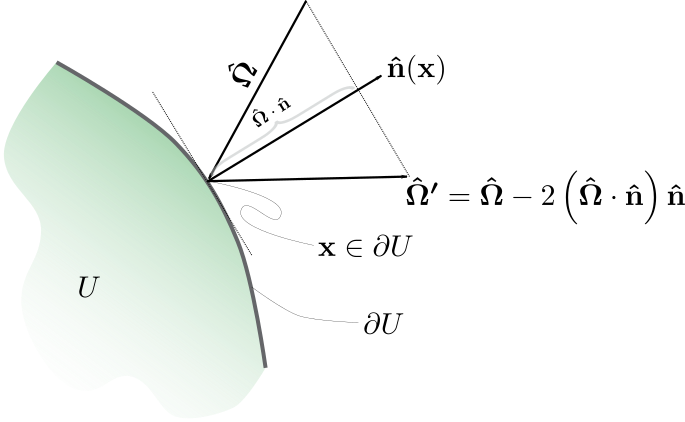
\includegraphics[width=0.6\linewidth]{transporte/reflejado}
\end{center}
\caption{\label{fig:reflejado}La dirección reflejada~$\omegaversor$ de la dirección incidente con respecto a la normal exterior~$\hat{\vec{n}}$ al dominio~$U$ en el punto~$\vec{x} \in \partial U$. Se cumple que~$\omegaversor \cdot \hat{\vec{n}} = -\omegaversor \cdot \hat{\vec{n}}$.}
\end{figure}

\medskip

En general, podemos fijar la corriente entrante al dominio a un cierto valor diferente de cero sólo si

\begin{enumerate}
 \item el término de fisión es nulo; ó
 \item el término de fisión es no nulo \emph{y} el término de fuentes es también no nulo
\end{enumerate}

En estos casos, podemos tener una condición de contorno general:

\begin{equation*}
\psi(\vec{x}, \omegaversor, E, t) = f(\vec{x}) \quad\quad \forall \vec{x} \notin \Gamma_V \cup \Gamma_M \wedge \omegaversor \cdot \hat{\vec{n}}(\vec{x}) < 0
\end{equation*}

\medskip

Notamos que en todos los casos las condiciones de contorno de la ecuación de transporte son de tipo Dirichlet.

\section{Aproximación de difusión} % WIP
\label{sec:difusion}

{\color{red} \lipsum[2]}

\subsection{Conservación de neutrones} % WIP

{\color{red} \lipsum[2]}

Comenzamos integrando la ecuación~\eqref{eq:transporteq} de transporte de neutrones sobre todos los ángulos~$\omegaversor$ para obtener

\begin{multline*}
\int_{4\pi} \frac{1}{v} \frac{\partial}{\partial t} \left[ \psi(\vec{x}, \omegaversor, E, t) \right] \, d\omegaversor
 + \int_{4\pi} \omegaversor \cdot \text{grad} \left[ \psi(\vec{x}, \omegaversor, E, t) \right] \, d\omegaversor \\
 + \int_{4\pi} \Sigma_t(\vec{x}, E) \cdot \psi(\vec{x}, \omegaversor, E, t) \, d\omegaversor
 = \int_{4\pi} q(\vec{x}, \omegaversor, E, t)  \, d\omegaversor
\end{multline*}

Utilizando la identidad de cálculo vectorial

\begin{equation*}
 \text{div}(\omegaversor \cdot \psi ) = \omegaversor \cdot \text{grad} \left( \psi \right) + \psi \cdot \text{div} ( \omegaversor ) 
\end{equation*}
%
y notando que~$\text{div} ( \omegaversor ) = 0$ porque las operaciones diferenciales actúan sólo sobre las coordenadas espaciales del vector~$\vec{x}$ y~$\omegaversor = [ \hat{\Omega}_x \, \hat{\Omega}_y \, \hat{\Omega}_z]^T$, podemos evaluar el segundo término como la divergencia de la integral sobre~$\omegaversor$ del producto escalar de la dirección por el flujo angular

\begin{multline*}
 \frac{1}{v} \frac{\partial}{\partial t} \left[ \int \psi(\vec{x}, \omegaversor, E, t) \, d\omegaversor \right]
 + \text{div} \left [ \int \left( \omegaversor  \cdot \psi(\vec{x}, \omegaversor, E, t)\right)\, d\omegaversor \right] \\
 + \Sigma_t(\vec{x}, E) \cdot \left[ \int \psi(\vec{x}, \omegaversor, E, t) \, d\omegaversor \right]
 = \int q(\vec{x}, \omegaversor, E, t) \, d\omegaversor
\end{multline*}
%

\medskip

Recordando las definiciones~\ref{def:flujoescalar} de flujo escalar~$\phi$ y~\ref{def:corriente} del vector corriente~$\vec{J}$,

\begin{align*}
\phi(\vec{x}, E, t) &= \int_{4\pi} \psi(\vec{x}, \omegaversor, E, t) \, d\omegaversor  \\
\vec{J}(\vec{x},E,t) &= \int_{4\pi} \left( \psi(\vec{x}, \omegaversor, E, t) \cdot \omegaversor \right) \, d\omegaversor
\end{align*}
% 
y definiendo una fuente escalar

\begin{equation}
\label{eq:Qgrande}
 Q(\vec{x}, E, t) = \int q(\vec{x}, \omegaversor, E, t) \, d\omegaversor
\end{equation}
%
obtenemos

\begin{equation}
\label{eq:conservacion}
 \frac{1}{v} \frac{\partial}{\partial t} \Big[ \phi(\vec{x}, E, t) \Big]
 + \text{div} \Big[ \vec{J}(\vec{x}, E, t) \Big]
 + \Sigma_t(\vec{x}, E) \cdot \phi(\vec{x}, E, t)
 = Q(\vec{x}, E, t) 
\end{equation}

Esta ecuación refleja la conservación del momento de orden cero del flujo angular de neutrones.

\subsection{Producciones} % WIP

El miembro derecho de la ecuación~\eqref{eq:conservacion} representa las producciones de neutrones, que como definimos en la ecuación~\eqref{eq:Qgrande}, es igual a la integral de las tres contribuciones individuales debidas a scattering, fisión y fuentes independientes:

\begin{align*}
 Q(\vec{x}, E, t) &= \int q(\vec{x}, \omegaversor, E, t) \, d\omegaversor \\
&= \int q_s(\vec{x}, \omegaversor, E, t) \, d\omegaversor
 + \int q_f(\vec{x}, \omegaversor, E, t) \, d\omegaversor
 + \int s(\vec{x}, \omegaversor, E, t) \, d\omegaversor \\
&= Q_s(\vec{x}, E, t) + Q_f(\vec{x}, E, t) + S(\vec{x}, E, t)
\end{align*}

\subsubsection{Fuente por scattering} % WIP

Para evaluar la contribución debida al scattering de neutrones integramos la ecuación~\eqref{eq:qsfacil} sobre todas las direcciones emergentes~$\omegaversor$:

% \begin{equation*}
%  Q_s(\vec{x}, E, t) = \bigintsss_{4\pi} \left( \int_{0}^{\infty} \left[ \Sigma_{s_\ell}(\vec{x}, E \rightarrow E^{\prime}) 
% \sum_{m=-\ell}^{\ell} \Psi_\ell^m (\vec{x}, E^{\prime}, t) \cdot Y_\ell^{m}(\omegaversor)  \right] \, dE^{\prime}
%  \right) \, d\omegaversor
% \end{equation*}
% 
% Para el caso particular de scattering linealmente anisotrópico, podemos utilizar la expresión~\eqref{eq:qslineal}
% 
% \begin{align*}
%  Q_s(\vec{x}, E, t) &= \bigintsss_{4\pi} 
% \frac{1}{4\pi} \left[ \int_{0}^{\infty} \Sigma_{s_0}(\vec{x}, E^{\prime} \rightarrow E) \cdot \phi(\vec{x}, E^{\prime}, t) \, dE^\prime \right]   \, d\omegaversor \\
% & \quad\quad + 
%  \bigintsss_{4\pi} \frac{3}{4\pi}
% \left[ \int_{0}^{\infty} \Sigma_{s_1}(\vec{x}, E^{\prime} \rightarrow E) \cdot \left(  \vec{J}(\vec{x},E^\prime,t) \cdot \omegaversor \right) \, dE^\prime \right]  \, d\omegaversor
% \end{align*}

\begin{multline*}
 Q_s(\vec{x}, E, t) = \bigintsss_{4\pi} \Bigg\{
\frac{1}{4\pi} \int_{0}^{\infty} \Sigma_{s_0}(\vec{x}, E^{\prime} \rightarrow E) \cdot \phi(\vec{x}, E^{\prime}, t) \, dE^\prime \\
+ \frac{3}{4\pi} \int_{0}^{\infty} \Sigma_{s_1}(\vec{x}, E^{\prime} \rightarrow E) \cdot \left(\vec{J}(\vec{x},E^{\prime},t) \cdot \omegaversor\right) \, dE^\prime  \\
+ \sum_{\ell=2}^\infty \bigintsss_{0}^{\infty}   \left[ \Sigma_{s_\ell}(\vec{x}, E^{\prime} \rightarrow E) 
\sum_{m=-\ell}^{\ell} \Psi_\ell^m (\vec{x}, E^{\prime}, t) \cdot Y_\ell^{m}(\omegaversor)  \right] \, dE^{\prime} \Bigg\} \, d\omegaversor
\end{multline*}

Todos los términos para~$\ell>1$ se anulan por ser integrales de funciones simétricas con respecto a~$\omegaversor$. Luego

\begin{equation}\label{eq:Qs}
Q_s(\vec{x}, E, t) = \int_{0}^{\infty} \Sigma_{s_0}(\vec{x}, E^{\prime} \rightarrow E)  \cdot \phi(\vec{x}, E^\prime, t) \, dE^\prime
\end{equation}


\subsubsection{Fuente por fisión} % WIP

El término que representa la fuente por fisión es la integral sobre todas las posibles direcciones del término de fuentes de fisión~$q_f$. Para el caso de la ecuación~\eqref{eq:qf}, que corresponde a un problema estacionario con fisión y fuente independiente (ver sección~\ref{sec:problemas}), tenemos

\begin{align}\label{eq:Qf}
Q_f(\vec{x},E,t) &= \bigintsss_{4\pi} \left[ \frac{\chi(E)}{4\pi} \int_{0}^{\infty} \nu\Sigma_f(\vec{x}, E^\prime) \cdot \phi(\vec{x}, E^\prime, t) \, dE^\prime \right] \, d\omegaversor \nonumber \\
&= \chi(E) \int_{0}^{\infty} \nu\Sigma_f(\vec{x}, E^\prime) \cdot \phi(\vec{x}, E^\prime, t) \, dE^\prime
\end{align}

\subsubsection{Fuente independiente} % WIP

La fuente independiente es directamente la integral sobre~$\omegaversor$ de la fuente independiente~$s(\vec{x}, \omegaversor, E, t)$:

\begin{equation}\label{eq:S}
 S(\vec{x},E,t) = \int_{4\pi} s(\vec{x}, \omegaversor, E, t) \,  d\omegaversor
  = s_0(\vec{x},E,t)
\end{equation}
%
es decir, el momento de orden cero de la expansión en armónicos esféricos de la fuente.



\subsection{Ley de Fick} % WIP
\label{sec:fick}

{\color{red}\lipsum[1]}

Como ya hemos mencionado, nuestro enfoque será primero que nada esencialmente matemático. Dejamos para el final del capítulo el análisis de las  implicaciones físicas que tienen las aproximaciones matemáticas que introducimos en esta sección para arribar a los resultados y conclusiones expuestos. Comencemos recordando la ecuación~\eqref{eq:transporteq}, explicitando los términos de fuentes por scattering~\eqref{eq:qs3}, fisión estacionaria~\eqref{eq:qf} y fuentes independientes:

\begin{multline}\label{eq:fick1}
 \frac{1}{v} \frac{\partial}{\partial t} \left[ \psi(\vec{x}, \omegaversor, E, t) \right]
 + \omegaversor \cdot \text{grad} \left[ \psi(\vec{x}, \omegaversor, E, t) \right]
 + \Sigma_t(\vec{x}, E) \cdot \psi(\vec{x}, \omegaversor, E, t)
 = \\
\bigintsss_{0}^{\infty} \sum_{\ell=0}^\infty \left[ \Sigma_{s_\ell}(\vec{x}, E^{\prime} \rightarrow E) 
\sum_{m=-\ell}^{\ell} \Psi_\ell^m (\vec{x}, E^{\prime}, t) \cdot Y_\ell^{m}(\omegaversor)  \right] \, dE^{\prime}
\\
+ \frac{\chi(E)}{4\pi} \int_{0}^{\infty} \nu\Sigma_f(\vec{x}, E^\prime) \cdot \phi(\vec{x}, E^\prime, t) \, dE^\prime
+ s(\vec{x}, \omegaversor, E, t)
\end{multline}

Multipliquemos esta ecuación escalar por el versor~$\omegaversor$ e integremos sobre todas las posibles direcciones para obtener una ecuación vectorial de dimensión tres:

\begin{multline}\label{eq:difusionporomega}
\int_{4\pi} \left( \frac{1}{v} \frac{\partial}{\partial t} \left[ \psi(\vec{x}, \omegaversor, E, t) \right] \cdot  \omegaversor \right) \, d\omegaversor
 +
\int_{4\pi} \left( \omegaversor \cdot \text{grad} \left[ \psi(\vec{x}, \omegaversor, E, t) \right] \cdot  \omegaversor \right) \, d\omegaversor
\\
 +
\int_{4\pi} \left( \Sigma_t(\vec{x}, E) \cdot \psi(\vec{x}, \omegaversor, E, t) \cdot  \omegaversor \right) \, d\omegaversor
 = 
\\
\bigintsss_{4\pi} \left( \int_{0}^{\infty} \sum_{\ell=0}^\infty  \left[ \Sigma_{s_\ell}(\vec{x}, E^{\prime} \rightarrow E) 
\sum_{m=-\ell}^{\ell} \Psi_\ell^m (\vec{x}, E^{\prime}, t) \cdot Y_\ell^{m}(\omegaversor)  \right] \, dE^{\prime}  \cdot  \omegaversor \right) \, d\omegaversor
\\
+ \int_{4\pi} \left( \frac{\chi(E)}{4\pi} \int_{0}^{\infty} \nu\Sigma_f(\vec{x}, E^\prime) \cdot \phi(\vec{x}, E^\prime, t) \, dE^\prime  \cdot  \omegaversor \right) \, d\omegaversor
+ \int_{4\pi} \left( s(\vec{x}, \omegaversor, E, t)  \cdot  \omegaversor \right) \, d\omegaversor
\end{multline}

Analicemos término a término esta expresión, teniendo en cuenta los desarrollos matemáticos que hemos realizado a lo largo de todo el capítulo. El primero corresponde a la derivada temporal de la corriente. En efecto

\begin{align}
\int_{4\pi} \left( \frac{1}{v} \frac{\partial}{\partial t} \left[ \psi(\vec{x}, \omegaversor, E, t) \right] \cdot  \omegaversor \right) \, d\omegaversor
& =
\frac{1}{v(E)} \frac{\partial}{\partial t}\left[ \int_{4\pi} \left( \psi(\vec{x}, \omegaversor, E, t) \cdot  \omegaversor \right) \, d\omegaversor \right]
\nonumber \\
& = \sqrt{\frac{m}{2E}} \frac{\partial}{\partial t}\Big[ \vec{J}(\vec{x}, E, t) \Big] \label{eq:difusion1}
\end{align}

\medskip

Dejemos para después el segundo término. El siguiente es el término de absorción total escrito en forma vectorial con respecto a la corriente

\begin{align}
\int_{4\pi} \left( \Sigma_t(\vec{x}, E) \cdot \psi(\vec{x}, \omegaversor, E, t) \cdot  \omegaversor \right) \, d\omegaversor
& =
\Sigma_t(\vec{x}, E) \cdot \int_{4\pi} \left( \psi(\vec{x}, \omegaversor, E, t) \cdot  \omegaversor \right) \, d\omegaversor \nonumber \\
& =
\Sigma_t(\vec{x}, E) \cdot \vec{J}(\vec{x}, E, t) \label{eq:difusion2}
\end{align}

\medskip


El término de scattering parece complicado, pero en realidad ya lo hemos resuelto al derivar la ecuación~\eqref{eq:recuperoj}. En primer lugar, partamos de la ecuación~\eqref{eq:qsfacil} multiplicada por~$\omegaversor$ e integrada en~$4\pi$:

\begin{multline*}
\bigintsss_{4\pi} \left[ \frac{1}{4\pi} \int_{0}^{\infty} \Sigma_{s_0}(\vec{x}, E^{\prime} \rightarrow E) \cdot \phi(\vec{x}, E^{\prime}, t) \cdot \omegaversor  \, dE^\prime \right] \, d\omegaversor \\
+ \bigintsss_{4\pi} \left[ \frac{3}{4\pi} \int_{0}^{\infty} \Sigma_{s_1}(\vec{x}, E^{\prime} \rightarrow E) \cdot \left(\vec{J}(\vec{x},E^{\prime},t) \cdot \omegaversor\right) \cdot \omegaversor\, dE^\prime \right] \, d\omegaversor  \\
+ \bigintsss_{4\pi}  \left\{ \sum_{\ell=2}^\infty \bigintsss_{0}^{\infty}   \left[ \Sigma_{s_\ell}(\vec{x}, E^{\prime} \rightarrow E) 
\sum_{m=-\ell}^{\ell} \Psi_\ell^m (\vec{x}, E^{\prime}, t) \cdot Y_\ell^{m}(\omegaversor) \cdot \omegaversor \right] \, dE^{\prime} \right\} \, d\omegaversor
\end{multline*}

En forma similar al argumento planteado en la página~\ref{pag:argumentoortogonal}, el primer término se anula por ser impar, y los términos de la sumatoria también se anulan por la propiedad de ortogonalidad de los armónicos esféricos (ecuación~\eqref{eq:ortogonalidadarmonicos}) y la ecuación~\eqref{eq:omegapropy}, que indica que~$\omegaversor$ es proporcional a~$Y_1^m(\omegaversor)$:

\begin{align*}
&= \frac{3}{4\pi} \bigintsss_{4\pi} \left\{ \int_0^\infty \Sigma_{s_1}(\vec{x},E^\prime \rightarrow E) \cdot \left( J_x \hat{\Omega}_x + J_y \hat{\Omega}_y + J_z \hat{\Omega}_z \right) \cdot
\begin{bmatrix}
 \hat{\Omega}_x \\ \hat{\Omega}_y \\ \hat{\Omega}_z
\end{bmatrix}
\, dE^\prime \right\}  \, d\omegaversor \\
&= \frac{3}{4\pi} \bigintsss_{4\pi}
\left\{ \int_0^\infty \Sigma_{s_1}(\vec{x},E^\prime \rightarrow E) \cdot
\begin{bmatrix}
 J_x \hat{\Omega}_x \hat{\Omega}_x +  J_y \hat{\Omega}_y \hat{\Omega}_x +  J_z \hat{\Omega}_z \hat{\Omega}_x \\
 J_x \hat{\Omega}_x \hat{\Omega}_y +  J_y \hat{\Omega}_y \hat{\Omega}_y +  J_z \hat{\Omega}_z \hat{\Omega}_y \\
 J_x \hat{\Omega}_x \hat{\Omega}_z +  J_y \hat{\Omega}_y \hat{\Omega}_z +  J_z \hat{\Omega}_z \hat{\Omega}_z
\end{bmatrix}
\, dE^\prime \right\}  \, d\omegaversor
\end{align*}
%
Teniendo además en cuenta la ecuación~\eqref{eq:43pi} (apéndice~\ref{ap:omega})

\begin{equation}\tag{\ref{eq:43pi}}
 \int_{4\pi} \hat{\Omega}_i \cdot \hat{\Omega}_j \, d\omegaversor = \frac{4\pi}{3} \cdot \delta_{ij}
\end{equation}
%
el término de scattering toma la inocua forma de


\begin{equation}\label{eq:difusion3}
 \int_0^\infty \Sigma_{s_1}(\vec{x},E^\prime \rightarrow E) \cdot \vec{J}(\vec{x}, E^\prime,t) \, dE^\prime
\end{equation}

\medskip

El siguiente es el término de fisiones, cuya integral se anula. En efecto,

\begin{equation}\label{eq:difusion4}
\bigintsss_{4\pi} \left( \frac{\chi(E)}{4\pi} \int_{0}^{\infty} \nu\Sigma_f(\vec{x}, E^\prime) \cdot \phi(\vec{x}, E^\prime, t) \, dE^\prime  \cdot  \omegaversor \right) \, d\omegaversor = 0
\end{equation}
%
ya que el integrando es una función impar de~${\omegaversor}$. En forma equivalente, en distribuciones angulares isotrópicas el único momento diferente de cero es el de orden~$\ell=0$.

\medskip

El término de fuentes independientes es igual a un vector cuyas componentes son los tres coeficientes de la expansión de la fuente en armónicos esféricos sobre el ángulo~$\omegaversor$:

\begin{align}
\int_{4\pi} s(\vec{x}, \omegaversor, E, t)  \cdot  \omegaversor \, d\omegaversor
& =
\sqrt{\frac{3}{4\pi}} \cdot 
\begin{bmatrix}
s_1^{1}(\vec{x},E,t) \\
s_1^{-1}(\vec{x},E,t) \\
s_1^{0}(\vec{x},E,t) \\
\end{bmatrix}
\nonumber \\
& =
\sqrt{\frac{3}{4\pi}} \cdot \vec{s}_1(\vec{x},E,t) \label{eq:difusion5}
\end{align}
%
a menos que las fuentes independientes sean isotrópicas, en cuyo caso estos momentos son nulos.

\medskip

El término que involucra el gradiente parece sencillo pero es el más complicado de la ecuación~\eqref{eq:difusionporomega}. En efecto,

{\color{red}Hacer bien las cuentas, hay que suponer que $\psi = \phi + 3J +$ términos superiores.}

\begin{equation}\label{eq:difusion6}
\int_{4\pi} \left( \omegaversor \cdot \text{grad} \left[ \psi(\vec{x}, \omegaversor, E, t) \right] \cdot  \omegaversor \right) \, d\omegaversor \simeq  \frac{1}{3}  \, \text{grad} \left[ \phi(\vec{x}, E,t ) \right]
\end{equation}


\medskip

Estamos entonces en condiciones de reunir todos estos términos (ecuaciones~\eqref{eq:difusion1}, \eqref{eq:difusion2}, \eqref{eq:difusion3}, \eqref{eq:difusion4}, \eqref{eq:difusion5} y \eqref{eq:difusion6}) y concluir que al multiplicar la ecuación~\eqref{eq:fick1} por~$\omegaversor$ e integrar en todas las posibles direcciones, obtenemos

% \begin{multline*}
%  \frac{1}{v}\frac{\partial \vec{J}}{\partial t} + \text{grad} \Big[ \phi(\vec{x}, E, t) \Big] + \Sigma_t(\vec{x},E) \cdot \vec{J}(\vec{x},E,t) =
% 3 \cdot \int_0^{\infty} \Sigma_{s_1}(\vec{x}, E^\prime \rightarrow E) \cdot \vec{J}(\vec{x},E^\prime,t) \, dE^\prime + \vec{s}_1(\vec{x},E,t)
% \end{multline*}


\begin{multline}
\frac{1}{v(E)} \frac{\partial}{\partial t}\Big[ \vec{J}(\vec{x}, E, t) \Big] + 
\frac{1}{3}  \, \text{grad} \left[ \phi(\vec{x}, E,t ) \right] +
\Sigma_t(\vec{x}, E) \cdot \vec{J}(\vec{x}, E, t)
= \\
\int_0^\infty \Sigma_{s_1}(\vec{x},E^\prime \rightarrow E) \cdot \vec{J}(\vec{x}, E^\prime,t) \, dE^\prime +
\sqrt{\frac{3}{4\pi}} \cdot \vec{s}_1(\vec{x},E,t) \label{eq:fickinterm1}
\end{multline}

A continuación vamos a hacer las siguientes tres suposiciones:

\begin{enumerate}
 \item que la fuente independiente es isotrópica por lo que el primer momento $\vec{s}_1(\vec{x}, E, t)$ es idénticamente nulo.

 \item que
\begin{equation*}
 \frac{3}{v}  \frac{\partial}{\partial t}\Big[ \vec{J}(\vec{x}, E, t) \Big] \ll \text{grad} \left[ \phi(\vec{x}, E,t ) \right]
\end{equation*}
%
lo que de hecho es cierto en el caso estacionario ya que $\partial \vec{J}/\partial t = 0$.

 \item que
\begin{equation}\label{eq:suposicionscattering}
\int_0^\infty \Sigma_{s_1}(\vec{x}, E^\prime \rightarrow E) \cdot \vec{J}(\vec{x}, E^\prime, t) \, dE^\prime
\simeq
\int_0^\infty \Sigma_{s_1}(\vec{x}, E \rightarrow E^\prime) \cdot \vec{J}(\vec{x}, E, t) \, dE^\prime
\end{equation}

El miembro izquierdo representa el in-scattering de neutrones de todas las energías mientras que el miembro derecho es el out-scattering de neutrones de energía~$E$ hacia todas las otras energías~$E^\prime$. Si la absorción es pequeña, estas dos expresiones se deberían balancear aproximadamente por lo que esta suposición es razonable.

\end{enumerate}

Volviendo a la ecuación~\eqref{eq:fickinterm1}, tenemos

\begin{align*}
\frac{1}{3}  \, \text{grad} \left[ \phi(\vec{x}, E,t ) \right] +
\Sigma_t(\vec{x}, E) \cdot \vec{J}(\vec{x}, E, t)
& =
\int_0^\infty \Sigma_{s_1}(\vec{x}, E \rightarrow E^\prime) \cdot \vec{J}(\vec{x}, E, t) \, dE^\prime  \\
& =
\int_0^\infty \Sigma_{s_1}(\vec{x}, E \rightarrow E^\prime) \, dE^\prime \cdot \vec{J}(\vec{x}, E, t)  \\
& =
\mu_0(\vec{x}, E) \int_0^\infty \Sigma_{s_0}(\vec{x}, E \rightarrow E^\prime) \, dE^\prime \cdot \vec{J}(\vec{x}, E, t)  \\
& =
\mu_0(\vec{x}, E) \cdot \Sigma_s(\vec{x}, E) \cdot \vec{J}(\vec{x}, E, t)
\end{align*}
%
donde en los últimos dos pasos hemos utilizado la ecuación~\eqref{eq:mu0}  y la sección eficaz \emph{total} de scattering~$\Sigma_s(\vec{x}, E)$. Con esta expresión podemos relacionar la corriente~$\vec{J}$ con el gradiente del flujo escalar~$\phi$ como

\begin{equation*}
 \vec{J}(\vec{x}, E, t) = -\frac{1}{3 \left[ \Sigma_t(\vec{x}, E) - \mu_0(\vec{x}, E) \cdot \Sigma_s(\vec{x},E) \right] } \cdot \text{grad} \left[ \phi(\vec{x}, E,t ) \right]
\end{equation*}

\begin{definicion}
El \emph{coeficiente de difusión}~$D$ definido como

\begin{equation*}
 D(\vec{x}, E) = \frac{1}{3 \left[ \Sigma_t(\vec{x}, E) - \mu_0(\vec{x}, E) \cdot \Sigma_s(\vec{x},E) \right] }
\end{equation*}
%
es tal que, si

 \begin{enumerate}
  \item la fuente independiente es isotrópica, $\vec{s}_1(\vec{x}, E, t)=0$;
  \item la variación temporal de la corriente es despreciable frente al gradiente del flujo escalar, $3/v  \cdot \partial \vec{J}/\partial t \ll \nabla \phi$;
  \item el in-scattering es similar al out-scattering, $\int \Sigma_{s_1}(E^\prime \rightarrow E) \cdot \vec{J}(E^\prime) \, dE^\prime
\simeq
\int \Sigma_{s_1}(E \rightarrow E^\prime) \cdot \vec{J}(E) \, dE^\prime$; y
  \item el flujo angular se puede ser aproximado como linealmente anisotrópico, $\psi \approx (\phi + 3\vec{J})/4\pi$
 \end{enumerate}
%
entonces se cumple la \emph{Ley de Fick}

\begin{equation}\label{eq:fick}
 \vec{J}(\vec{x}, E, t) \simeq - D(\vec{x}, E) \cdot \text{grad} \left[ \phi(\vec{x}, E, t) \right]
\end{equation}
%
según la cual el vector corriente~$\vec{J}$ es proporcional a menos el gradiente del flujo escalar~$\phi$ a través de un coeficiente de difusión~$D$.
\end{definicion}

La ley de Fick refleja la conservación del momento de orden uno del flujo angular de neutrones en forma aproximada.




\subsection{La ecuación de difusión} % WIP

Podemos combinar los dos resultados de las secciones anteriores (conservación de momentos de orden cero y uno) teniendo en cuenta las ecuaciones~\eqref{eq:conservacion}, \eqref{eq:Qs}, \eqref{eq:Qf}, \eqref{eq:S} y~\eqref{eq:fick} para obtener finalmente la celebrada ecuación de difusión de neutrones

\begin{multline}\label{eq:difusion}
 \sqrt{\frac{m}{2E}} \frac{\partial}{\partial t} \Big[ \phi(\vec{x}, E, t) \Big]
 - \text{div} \Big[ D(\vec{x}, E) \cdot \text{grad} \left[ \phi(\vec{x}, E, t) \right] \Big]
 + \Sigma_t(\vec{x}, E) \cdot \phi(\vec{x}, E, t)
 = \\
\int_{0}^{\infty} \Sigma_{s_0}(\vec{x}, E^{\prime} \rightarrow E)  \cdot \phi(\vec{x}, E^\prime, t) \, dE^\prime +
\chi(E) \int_{0}^{\infty} \nu\Sigma_f(\vec{x}, E^\prime) \cdot \phi(\vec{x}, E^\prime, t) \, dE^\prime
+ s_0(\vec{x}, E, t)
\end{multline}
%
que es una ecuación de segundo orden sobre el espacio (los operadores divergencia y gradiente operan sólo sobre las coordenadas espaciales) y de primer orden sobre el tiempo para la incógnita~$\phi(\vec{x}, E,t)$. Las secciones eficaces~$\Sigma_t$, y~$\nu\Sigma_f$ son funciones conocidas del espacio~$\vec{x}$ y la energía~$E$, al igual que el coeficiente de difusión~$D(\vec{x},E)$. La sección eficaz diferencial de scattering~$\Sigma_{s_0}$ es el momento de orden cero de la expansión en polinomios de Legendre de la sección eficaz de scattering diferencial~$\Sigma_s$ para dispersión desde la energía~$E^\prime$ a la energía~$E$, también conocida para todo~$\vec{x}$. La distribución~$\chi(E)$ es el espectro de fisión en función de la energía~$E$, $s_0$ es el momento de orden cero en la expansión de la fuente independiente en armónicos esféricos y~$m$ es la masa en reposo del neutrón, todos parámetros que asumimos son conocidos.


\subsection{Condiciones de contorno} % WIP
\label{sec:bcdifusion}

La ecuación de difusión es elíptica sobre las coordenadas espaciales por lo que debemos especificar, además de las condiciones iniciales apropiadas en el caso transitorio, condiciones de contorno en toda la frontera~$\partial U$ del dominio espacial. Tal como discutimos en la sección~\ref{sec:bctransporte}, éstas pueden ser

 \begin{enumerate}
  \item de Dirichlet donde especificamos el valor del flujo escalar~$\phi$ en $\Gamma_D \subset \partial U$;
  \item de Neumann donde fijamos el valor de la derivada normal~$\partial \phi/\partial n$ en~$\Gamma_N \subset \partial U$; ó bien
  \item de Robin donde damos una combinación lineal del flujo y de la derivada normal en~$\Gamma_R \subset \partial U$.
 \end{enumerate}

Debe cumplirse que $\Gamma_D \cap \Gamma_N \cap \Gamma_R = \emptyset$ y que $\Gamma_D \cup \Gamma_N \cup \Gamma_R = \partial U$.

\medskip

Dada una superficie diferencial cuya normal exterior es~$\hat{\vec{n}}$, tasa de neutrones entrante por unidad de área a través de dicha superficie está dada por la ecuación~\eqref{eq:jnegativa} de la definición~\ref{def:corriente}:

\begin{equation}\tag{\ref{eq:jnegativa}}
\ J_n^-(\vec{x},E,t) = \int_{\omegaversor \cdot \hat{\vec{n}} < 0} \psi(\vec{x}, \omegaversor, E, t) \left(\omegaversor \cdot \hat{\vec{n}}\right) d\omegaversor 
\end{equation}

Despreciando los términos para~$\ell \geq 2$ en la ecuación~\eqref{eq:psi1}, podemos estimar esta corriente como

\begin{align*}
J_n^-(\vec{x},E,t) & \approx \int_{\omegaversor \cdot \hat{\vec{n}} < 0} \frac{1}{4\pi} \left [ \phi(\vec{x}, E, t) + 3 \, \vec{J}(\vec{x}, E, t) \cdot \omegaversor \right]  \left(\omegaversor \cdot \hat{\vec{n}}\right) d\omegaversor
\\
& \approx \frac{1}{4\pi} \phi(\vec{x}, E, t) \int_{0}^{-1} \mu^\prime \cdot 2\pi\, d\mu^\prime + 
\frac{3}{4\pi}  \int_{\omegaversor \cdot \hat{\vec{n}} < 0} \Big[ \vec{J}(\vec{x}, E, t) \cdot \omegaversor \Big] \cdot \left(\omegaversor \cdot \hat{\vec{n}}\right) d\omegaversor \\
& \approx \frac{1}{4\pi} \phi(\vec{x}, E, t) \cdot 2\pi \cdot \frac{1}{2} + \frac{3}{4\pi} \cdot \Big[ \vec{J}(\vec{x}, E, t) \cdot \hat{\vec{n}} \Big] \cdot \left(- \frac{2}{3} \pi \right)  \\
& \approx \frac{1}{4} \phi(\vec{x}, E, t) - \frac{1}{2} \Big[ \vec{J}(\vec{x}, E, t) \cdot \hat{\vec{n}} \Big]
\end{align*}
%
donde hemos usado la ecuación~\eqref{eq:43pi} sobre una semi-esfera unitaria para resolver la segunda integral del miembro derecho. A la luz de la ley de Fick dada por la ecuación~\eqref{eq:fick}, podemos escribir

\begin{align*}
J_n^-(\vec{x},E,t) & \approx \frac{1}{4} \phi(\vec{x}, E, t) + \frac{1}{2} D(\vec{x}, E) \cdot \Big[ \text{grad} \big[ \phi(\vec{x}, E, t)\big]  \cdot \hat{\vec{n}} \Big] \\
& \approx \frac{\phi(\vec{x}, E, t)}{4}  + \frac{D(\vec{x}, E)}{2}  \cdot \frac{\partial \phi}{\partial n}
\end{align*}
%
lo que nos da una expresión para definir las condiciones de contorno de la ecuación de difusión.

\begin{definicion}
\label{def:ccvacuumdif}
En forma análoga a la definición~\ref{def:ccvacuum}, llamamos \emph{condición de contorno de vacío} a la situación en la cual la corriente entrante a través de una porción de la frontera~$\partial U$ es cero, con lo que se debe cumplir:

\begin{equation}\label{eq:ccvacuumdif}
\phi(\vec{x}, E, t)  + 2 \cdot D(\vec{x}, E) \cdot \frac{\partial \phi}{\partial n} = 0
\end{equation}

Definimos el conjunto~$\Gamma_V \in \partial U$ como el lugar geométrico de todos los puntos~$\vec{x} \in \partial U$ donde imponemos esta condición de contorno. Esta condición es de tipo Robin ya que se da el valor de una combinación lineal de la incógnita~$\phi$ y de su derivada normal~$\partial \phi/\partial n$.
\end{definicion}

\begin{definicion}
\label{def:ccmirrordif}
En forma análoga a la definición~\ref{def:ccmirror}, llamamos \emph{condición de contorno de reflexión o de simetría} cuando la corriente neta entrante en el punto~$\vec{x} \in \partial U$ es igual a cero. En este caso, por la ley de Fick~\eqref{eq:fick}, debe anularse la derivada normal del flujo escalar evaluada en~$\vec{x}$:

\begin{equation*}
\text{grad} \big[ \phi(\vec{x}, E, t)\big]  \cdot \hat{\vec{n}} = \frac{\partial \phi}{\partial n} = 0
\end{equation*}

Esta es una condición de tipo Neumann. Definimos el conjunto~$\Gamma_M \in \partial U$ como el lugar geométrico de todos los puntos~$\vec{x} \in \partial U$ donde imponemos esta condición de contorno.
\end{definicion}


\medskip

Para el problema de difusión, a veces se suele utilizar una tercera condición de contorno basada en la idea que sigue. Si extrapolamos linealmente el flujo escalar~$\phi$ una distancia~$d$ en la dirección de la normal externa~$\hat{\vec{n}}$ en la frontera~$\partial U$ mediante una expansión de Taylor a primer orden, tenemos

\begin{equation*}
 \left. \phi \big(\vec{x} + d(\vec{x}, E) \cdot \hat{\vec{n}}, E, t \big) \right|_{\vec{x} \in \partial U} \approx \phi(\vec{x}, E, t) + \frac{\partial \phi}{\partial n} \cdot d(\vec{x}, E)
\end{equation*}

\begin{figure}
\begin{center}
 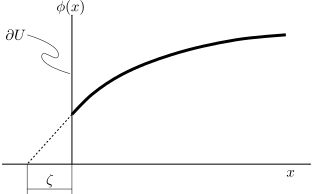
\includegraphics{transporte/cc}
\end{center}
\caption{\label{fig:cc} El flujo escalar~$\phi(\vec{x}, E,t)$ extrapolado linealmente se anula a una distancia~$d(\vec{x},E)= 2D(\vec{x},E)$ en una condición de contorno tipo vacío de la ecuación de difusión.}
\end{figure}

Si se cumple la condición de contorno~\eqref{eq:ccvacuumdif}, entonces el flujo escalar extrapolado se anula en $\vec{x} + 2 \cdot D(\vec{x}, E) \cdot \hat{\vec{n}}$, como ilustramos en la figura~\ref{fig:cc}. Si~$D(\vec{x}, E)$ es mucho menor que el tamaño característico del dominio~$U$ entonces podemos aproximar~$d \approx 0$.

\begin{definicion}
\label{def:ccnulldif}
Llamamos \emph{condición de contorno de flujo nulo} cuando el flujo escalar~$\phi$ se anula un punto~$\vec{x} \in \partial U$:

\begin{equation*}
\phi(\vec{x}, E, t) = 0
\end{equation*}

Definimos el conjunto~$\Gamma_N \in \partial U$ como el lugar geométrico de todos los puntos~$\vec{x} \in \partial U$ donde imponemos esta condición de contorno. Matemáticamente esta condición es de tipo Dirichlet.
\end{definicion}


\medskip

La condición de contorno más general que podemos dar es una combinación lineal del flujo más su derivada normal en la frontera del dominio:

\begin{equation*}
 a(\vec{x}) \cdot \phi(\vec{x},E,t) + b(\vec{x}) \cdot \frac{\partial \phi}{\partial n} = c(\vec{x})
\end{equation*}

Debemos notar que~$c(\vec{x})$ sólo puede ser diferente de cero si el término de fisión es nulo o si tanto el término de fisión como la fuente independiente no son nulos. Para dar una condición de reflectividad de un albedo~$\beta(\vec{x}, E)$ debemos dar como condición de contorno

\begin{equation*}
\begin{cases}
 a(\vec{x}) &= 1 \\
 b(\vec{x}) &= \displaystyle - \frac{1}{2\cdot D(\vec{x},E)} \cdot \frac{1 - \beta(\vec{x}, E)}{1 + \beta(\vec{x},E)} \\
 c(\vec{x}) &= 0 \\
\end{cases}
 \end{equation*}



\subsection{Validez de las suposiciones y aproximaciones} % WIP

Analicemos en esta sección qué implicaciones físicas tienen las suposiciones y aproximaciones matemáticas que hemos utilizado para arribar a la ecuación de difusión~\eqref{eq:difusion}. 

{\color{red} aún cuando no se cumplan todas, todavía se puede obtener una relación entre el gradiente del flujo y la corriente}


\section{Problemas de estado estacionario} % WIP
\label{sec:problemas}

Si bien hasta el momento hemos mantenido por completitud la dependencia temporal explícitamente en los flujos y corrientes, en este tesis estamos interesado principalmente en problemas de estado estacionario. Para ello, tenemos que anular los términos que involucren derivadas parciales con respecto al tiempo en las ecuaciones tanto de transporte como de difusión de neutrones. Esto cambia las propiedades matemáticas de las ecuaciones y por lo tanto la forma en la cual debemos resolverlas. Vamos a particularizar la ecuación de transporte~\eqref{eq:transporte} y la de difusión~\eqref{eq:difusion} para tres casos:

\begin{itemize}
 \item Medio no multiplicativo con fuentes independientes;
 \item Medio multiplicativo con fuentes independientes; y
 \item Medio multiplicativo sin fuentes independientes.
\end{itemize}

Debemos anular todos los términos de las derivadas temporales y eliminar todas las dependencias con respecto a la variable~$t$.
En cada caso discutimos las posibles condiciones de contorno necesarias para completar la formulación matemática.


\subsection{Medio no multiplicativo con fuentes independientes} % WIP

Un medio no multiplicativo es aquel que no contiene núcleos capaces de fisionar. Cada neutrón que encontremos en el medio debe entonces provenir de una fuente externa~$s$. Además de eliminar la derivada temporal y la dependencia con el tiempo, no tenemos en cuenta el término de fisión. Luego la ecuación de transporte~\eqref{eq:transporte} queda

\begin{multline}
\label{eq:transportenmfi}
\omegaversor \cdot \text{grad} \left[ \psi(\vec{x}, \omegaversor, E) \right]
 + \Sigma_t(\vec{x}, E) \cdot \psi(\vec{x}, \omegaversor, E) = \\
\int_{0}^{\infty} \int_{4\pi} \Sigma_s(\vec{x}, \omegaprimaversor \rightarrow \omegaversor, E^\prime \rightarrow E) \cdot \psi(\vec{x}, \omegaprimaversor, E^\prime) \, d\omegaprimaversor \, dE^\prime
+ s(\vec{x}, \omegaversor, E)
\end{multline}
%
y la de difusión~\eqref{eq:difusion}

\begin{multline}
\label{eq:difusionnmfi}
 - \text{div} \Big[ D(\vec{x}, E) \cdot \text{grad} \left[ \phi(\vec{x}, E) \right] \Big]
 + \Sigma_t(\vec{x}, E) \cdot \phi(\vec{x}, E)
 = \\
\int_{0}^{\infty} \Sigma_{s_0}(\vec{x}, E^{\prime} \rightarrow E)  \cdot \phi(\vec{x}, E^\prime) \, dE^\prime
+ s_0(\vec{x}, E)
\end{multline}

Para obtener soluciones de flujo no nula o bien la fuente no se debe anular idénticamente en el dominio o bien las condiciones de contorno deben ser no homogéneas. Si las secciones eficaces (incluyendo el coeficiente de difusión) dependen explícitamente de la posición~$\vec{x}$ y no dependen del flujo~$\psi$ o~$\phi$, entonces ambas ecuaciones~\eqref{eq:transportenmfi} y~\eqref{eq:difusionnmfi} son lineales. Al reordenar términos y discretizar el problema (capítulo~\ref{cap:esquemas}) obtendremos un sistema de ecuaciones algebraicas lineales que puede ser escrito en forma matricial como

\begin{equation*}
 A \vec{u} = \vec{b}
\end{equation*}
%
donde~$A \in \mathbb{R}^{n \times n}$ es una matriz cuadrada que contiene información sobre  la discretización de los operadores diferenciales e integrales de la ecuación,  $\vec{b} \in \mathbb{R}^n$ es un vector que contiene la versión discretizada de la fuente  independiente~$s$. La información sobre las condiciones de contorno pueden estar incluidas bien en~$A$ o bien en~$\vec{b}$, dependiendo del tipo de condición. Incluso las condiciones de tipo Robin tienen información tanto en~$A$ como en~$\vec{b}$. El vector~$\vec{u} \in \mathbb{R}^n$ es la incógnita, que luego de resolver el sistema permitirá estimar la función~$\psi$ ó~$\phi$ en  función de~$\vec{x}$, $E$ y eventualmente~$\omegaversor$.

{\color{red}ejemplo problema de la sección XXX}

{\color{red}caso no lineal (manual de milonga)}


\subsection{Medio multiplicativo con fuentes independientes} % WIP
\label{sec:multiplicativoconfuente}

Si además de contar con fuentes independientes de fisión el medio contiene material multiplicativo, entonces los neutrones pueden provenir tanto de las fuentes como de las fisiones. En este caso, tenemos que tener en cuenta la fuente de fisión, cuyo valor en la posición~$\vec{x}$ es proporcional al flujo escalar en~$\vec{x}$. En la sección~\ref{sec:fision} indicamos que debemos utilizar expresiones diferentes para la fuente de fisión dependiendo de si estamos resolviendo un problema transitorio o estacionario. Si bien sólo una fracción~$\beta$ de todos los netrones nacidos por fisión se generan en forma instantánea, en en estado estacionario debemos también sumar el resto de los~$(1-\beta)$ como fuente de fisión ya que suponemos el estado encontrado es un equilibrio instante a instante dado por los~$\beta$ neutrones prompt y $(1-\beta)$ neutrones retardados que provienen de fisiones operando desde~$t=-\infty$. La fuente de fisión para un medio multiplicativo con fuente independiente por unidad de ángulo sólido, recordando que la fisión es isotrópica, es

\begin{equation}\label{eq:fisionconfuentes}
q_s(\vec{x}, \omegaversor, E) = \frac{\chi(E)}{4\pi} \int_{0}^{\infty} \int_{4\pi} \nu\Sigma_f(\vec{x}, E^\prime) \cdot \psi(\vec{x}, \omegaprimaversor, E^\prime) \, d\omegaprimaversor \, dE^\prime  
\end{equation}


La expresión matemática de la ecuación de transporte~\eqref{eq:transporte} para este caso es  

\begin{multline}
\label{eq:transportemmfi}
 \omegaversor \cdot \text{grad} \left[ \psi(\vec{x}, \omegaversor, E) \right]
 + \Sigma_t(\vec{x}, E) \cdot \psi(\vec{x}, \omegaversor, E) = \\
 \int_{0}^{\infty} \int_{4\pi} \Sigma_s(\vec{x}, \omegaprimaversor \rightarrow \omegaversor, E^\prime \rightarrow E) \cdot \psi(\vec{x}, \omegaprimaversor, E^\prime) \, d\omegaprimaversor \, dE^\prime \\
+ \frac{\chi(E)}{4\pi} \int_{0}^{\infty} \int_{4\pi} \nu\Sigma_f(\vec{x}, E^\prime) \cdot \psi(\vec{x}, \omegaprimaversor, E^\prime) \, d\omegaprimaversor \, dE^\prime 
+ s(\vec{x}, \omegaversor, E)
\end{multline}
%
y de la ecuación de difusión~\eqref{eq:difusion} es


\begin{multline}
\label{eq:difusionmmfi}
 - \text{div} \Big[ D(\vec{x}, E) \cdot \text{grad} \left[ \phi(\vec{x}, E) \right] \Big]
 + \Sigma_t(\vec{x}, E) \cdot \phi(\vec{x}, E)
 = \\
\int_{0}^{\infty} \Sigma_{s_0}(\vec{x}, E^{\prime} \rightarrow E)  \cdot \phi(\vec{x}, E^\prime) \, dE^\prime +
\chi(E) \int_{0}^{\infty} \nu\Sigma_f(\vec{x}, E^\prime) \cdot \phi(\vec{x}, E^\prime) \, dE^\prime
+ s_0(\vec{x}, E)
\end{multline}

El tipo de problema discretizado es esencialmente similar a medio no multiplicativo con fuentes de la sección anterior, sólo que ahora la matriz~$A$ tiene información sobre las fuentes de fisión. Estos casos se encuentran al estudiar sistemas subcríticos como por ejemplo piletas de almacenamiento de combustibles gastados o procedimientos de puesta a crítico de reactores. 


\subsection{Medio multiplicativo sin fuentes independientes} % WIP

En el caso en que todos los neutrones provengan de fisiones y no existan fuentes independientes, en principio deberíamos anular las fuentes~$s$ y~$s_0$ de las ecuaciones~\eqref{eq:transportemmfi} y~\eqref{eq:difusionmmfi}, respectivamente. Sin embargo esta operación dejaría un problema matemático mal condicionado. En efecto, sin fuentes externas la ecuación a resolver (sea transporte o difusión) es homogénea. La probabilidad de que dada una geometría y un conjunto de secciones eficaces macroscópicas (i.e. un modelo matemático de un reactor) la ecuación arroje un flujo no trivial balanceando exactamente todos los términos de la ecuación (i.e. que el reactor esté exactamente crítico) es cero. Para tener una solución matemática (y físicamente) razonable, debemos agregar al menos un parámetro real que permita ajustar uno o más términos en forma continua. Por ejemplo podríamos escribir las secciones eficaces en función de un parámetro geométrico (la posición de una barra de control) y/o físico (la concentración media de boro en el moderador).

Hay un parámetro real que además de permitir encontrar una solución no trivial para cualquier conjunto físicamente razonable de geometrías y secciones eficaces, nos da una idea de qué tan lejos se encuentra el modelo de la criticidad. El procedimiento consiste en dividir el término de fisiones por un número real~$k_\text{eff}$, para obtener

\begin{multline}
\label{eq:transportemm}
 \omegaversor \cdot \text{grad} \left[ \psi(\vec{x}, \omegaversor, E) \right]
 + \Sigma_t(\vec{x}, E) \cdot \psi(\vec{x}, \omegaversor, E) = \\
 \int_{0}^{\infty} \int_{4\pi} \Sigma_s(\vec{x}, \omegaprimaversor \rightarrow \omegaversor, E^\prime \rightarrow E) \cdot \psi(\vec{x}, \omegaprimaversor, E^\prime) \, d\omegaprimaversor \, dE^\prime \\
+ \frac{1}{k_\text{eff}} \cdot \frac{\chi(E)}{4\pi} \int_{0}^{\infty} \int_{4\pi} \nu\Sigma_f(\vec{x}, E^\prime) \cdot \psi(\vec{x}, \omegaprimaversor, E^\prime) \, d\omegaprimaversor \, dE^\prime 
\end{multline}
%
y la de difusión~\eqref{eq:difusion} como

\begin{multline}
\label{eq:difusionmm}
 - \text{div} \Big[ D(\vec{x}, E) \cdot \text{grad} \left[ \phi(\vec{x}, E) \right] \Big]
 + \Sigma_t(\vec{x}, E) \cdot \phi(\vec{x}, E)
 = \\
\int_{0}^{\infty} \Sigma_{s_0}(\vec{x}, E^{\prime} \rightarrow E)  \cdot \phi(\vec{x}, E^\prime) \, dE^\prime +
\frac{1}{k_\text{eff}} \cdot \chi(E) \int_{0}^{\infty} \nu\Sigma_f(\vec{x}, E^\prime) \cdot \phi(\vec{x}, E^\prime) \, dE^\prime
\end{multline}

La utilidad del factor~$k_\text{eff}$ queda reflejada en la siguiente definición.

\begin{definicion}
Llamamos \emph{factor de multiplicación efectivo} al número real~$k_\text{eff}$ por el cual dividimos la fuente de fisiones de las ecuaciones que modelan un medio multiplicativo sin fuentes externas. Al nuevo medio al cual se le han dividido sus fuentes de fisión por~$k_\text{eff}$ lo denominamos \emph{reactor crítico asociado en~$k$}. Si~$k_\text{eff}>1$ entonces el reactor original estaba supercrítico ya que hubo que disminuir sus fisiones para encontrar una solución no trivial, y viceversa. El flujo solución de las ecuaciones es el flujo del reactor crítico asociado en~$k$ y no del original, ya que si el original no estaba crítico entonces éste no tiene solución estacionaria.
\end{definicion}

En este caso, al no haber fuentes independientes sólo quedan términos homogéneos. Sin embargo, ahora habrá algunos términos multiplicados por le coeficiente~$1/k_\text{eff}$ y otros no. Si las secciones eficaces dependen sólo de la posición~$\vec{x}$ en forma explícita y no a través del flujo, entonces el problema es lineal y al separar en ambos miembros estos dos tipos de términos obtendremos una formulación discretizada de la forma

\begin{equation}
 A \vec{u} = \lambda B \vec{u}
\end{equation}
%
conformando un problema de autovalores generalizado, donde el autovalor~$\lambda$ dará una idea de la criticidad del reactor y el autovector~$\vec{u}$ la distribución de flujo del reactor crítico asociado en~$k$.
Si~$B$ contiene los términos de fisión entonces~$\lambda = 1/k_\text{eff}$ y si~$A$ es la que contiene los términos de fisión, entonces~$\lambda = k_\text{eff}$.
En general, para matrices de~$n \times n$ habrá~$n$ pares autovalor-autovector. Más aún, tanto el autovalor como los elementos del autovector son en general complejos. 
Sin embargo se puede probar~\cite{henry} {\color{red}había una demostración del caso discretizado? chaboncito?} que, para el caso~$\lambda=1/k_\text{eff}$ ($\lambda=k_\text{eff}$), 

\begin{enumerate}\label{enum:properties}
 \item hay un único autovalor positivo real que es mayor (menor) en magnitud que el resto de los autovalores,
 \item todos los elementos del autovector correspondiente a dicho autovalor son reales y tienen el mismo signo, y
 \item todos los otros autovectores o bien tienen al menos un elemento igual a cero o tienen elementos que difieren en su signo
\end{enumerate}

\medskip

Debemos notar que éste un problema matemáticamente homogéneo. Esta característica define dos propiedades importantes. La primera es que el autovector (es decir el flujo) está definido a menos de una constante multiplicativa y es independiente del factor de multiplicación~$k_\text{eff}$. Para poder comparar soluciones debemos normalizar el flujo de alguna manera. Usualmente se define la potencia térmica total~$P$ del reactor y normalizamos el flujo de forma tal que

\begin{equation*}
 P = \int_{V} \int_0^\infty e\Sigma_f(\vec{x}, E) \cdot \phi(\vec{x}, E) \, dE \, d^3\vec{x}
\end{equation*}
%
donde~$e\Sigma_f$ es el producto de la energía liberada en una fisión individual por la sección eficaz de fisión. Debemos remarcar que si~$P$ es la potencia térmica instantánea, entonces~$e\Sigma_f$ debe incluir sólo las contribuciones energéticas de los productos de fisión instantáneos. Si~$P$ es la potencia términca total, entonces~$e\Sigma_f$ debe tener en cuenta todas las contribuciones, incluyendo aquellas debidas a efectos retardados de los productos de fisión.

La segunda propiedad es que las condiciones de contorno también deben ser homogéneas. Es decir, no es posible fijar valores de flujo o corrientes diferentes de cero. De todas formas, las condiciones de contorno definidas con nombre y apellido en las secciones~\ref{sec:bctransporte} ~\ref{sec:bcdifusion} son homogéneas por lo que aplican perfectamente para los medios multiplicativos sin fuentes externas.

{\color{red} no linealidades, ya no es cierto que el flujo es cualquier cosa}

% Este caso donde el medio es multiplicativo y no existen fuentes independientes aplica a la mayor cantidad de problemas de interés de la física de reactores. El factor de multiplicación efectiva~$k_\text{eff}$ da una idea de qué tan cerca de la criticidad está el reactor propuesto y el flujo obtenido es una aproximación de la distribución de flujo que tendría un hipotético reactor 


\section{Esquema de solución multiescala} % WIP
\label{sec:multiescala}

Si bien la ecuación de transporte~\eqref{eq:transporte} describe completamente la interacción de neutrones con la materia, los cambios en las secciones eficaces con la energía de los neutrones (figura~\ref{fig:xs})  
Los coeficientes de la ecuación de transporte son esencialmente las secciones eficaces macroscópicas.

\subsection{Evaluación y procesamiento de secciones eficaces} % TBD
\label{sec:evaluacionxs}

% En este paso del esquema de solución obtenemos, a partir de datos experimentales, las secciones eficaces microscópicas de los isótopos involucrados en el problema para diferentes temperaturas y discretizados en una cierta cantidad de energías del orden de la centena. Primeramente debemos ajustar modelos de dependencia de las secciones eficaces microscópicas 
% 
% Los datos nucleares correspondientes a los diferentes nucleídos involucrados en un cierto caso deben ser sintetizados ajustando modelos a valores experimentales, resolviendo potenciales inconsistencias en las mediciones, agrupando isótopos similares y teniendo en cuenta además efectos como la dinámica molecular para neutrones de baja energía. En este proceso de evaluación obtenemos un conjunto de datos que se denominan datos nucleares evaluados. Luego debemos procesar estos datos para obtener bibliotecas apropiadas para el cálculo de celda, tanto en su formato como en su contenido (agrupación por isótopo o por material, energías interpoladas o grupos discretos, tratamientos de resonancias, temperaturas, etc.). 
% 
% Un trabajo reciente de alta calidad y que debe servir como referencia de trabajos desarrollados en el país en esta escala de cálculo es la tesis doctoral de Ignacio Marquez Damián {\color{red}citar}.
% 
% {\color{red} ecuaciones lindas de nacho}
% por ejemplo, módulo THERMR + cálculo de matrices de scattering expandidas hasta $\ell$
% 
% {\color{red}poner una figura de la tesis de nacho}


\subsection{Cálculo a nivel celda} % TBD
\label{sec:celda}

% {\color{red}citar a chaco}

\subsection{Cálculo a nivel núcleo} % TBD

{\color{red}
\lipsum[14]

\begin{equation}
 R \cdot \vec{\phi} = \frac{1}{k_\text{eff}} F \cdot \vec{\phi}
\end{equation}

\lipsum[15]
}



